% Options for packages loaded elsewhere
\PassOptionsToPackage{unicode}{hyperref}
\PassOptionsToPackage{hyphens}{url}
%
\documentclass[
]{article}
\usepackage{amsmath,amssymb}
\usepackage{iftex}
\ifPDFTeX
  \usepackage[T1]{fontenc}
  \usepackage[utf8]{inputenc}
  \usepackage{textcomp} % provide euro and other symbols
\else % if luatex or xetex
  \usepackage{unicode-math} % this also loads fontspec
  \defaultfontfeatures{Scale=MatchLowercase}
  \defaultfontfeatures[\rmfamily]{Ligatures=TeX,Scale=1}
\fi
\usepackage{lmodern}
\ifPDFTeX\else
  % xetex/luatex font selection
\fi
% Use upquote if available, for straight quotes in verbatim environments
\IfFileExists{upquote.sty}{\usepackage{upquote}}{}
\IfFileExists{microtype.sty}{% use microtype if available
  \usepackage[]{microtype}
  \UseMicrotypeSet[protrusion]{basicmath} % disable protrusion for tt fonts
}{}
\makeatletter
\@ifundefined{KOMAClassName}{% if non-KOMA class
  \IfFileExists{parskip.sty}{%
    \usepackage{parskip}
  }{% else
    \setlength{\parindent}{0pt}
    \setlength{\parskip}{6pt plus 2pt minus 1pt}}
}{% if KOMA class
  \KOMAoptions{parskip=half}}
\makeatother
\usepackage{xcolor}
\usepackage[margin=1in]{geometry}
\usepackage{color}
\usepackage{fancyvrb}
\newcommand{\VerbBar}{|}
\newcommand{\VERB}{\Verb[commandchars=\\\{\}]}
\DefineVerbatimEnvironment{Highlighting}{Verbatim}{commandchars=\\\{\}}
% Add ',fontsize=\small' for more characters per line
\usepackage{framed}
\definecolor{shadecolor}{RGB}{248,248,248}
\newenvironment{Shaded}{\begin{snugshade}}{\end{snugshade}}
\newcommand{\AlertTok}[1]{\textcolor[rgb]{0.94,0.16,0.16}{#1}}
\newcommand{\AnnotationTok}[1]{\textcolor[rgb]{0.56,0.35,0.01}{\textbf{\textit{#1}}}}
\newcommand{\AttributeTok}[1]{\textcolor[rgb]{0.13,0.29,0.53}{#1}}
\newcommand{\BaseNTok}[1]{\textcolor[rgb]{0.00,0.00,0.81}{#1}}
\newcommand{\BuiltInTok}[1]{#1}
\newcommand{\CharTok}[1]{\textcolor[rgb]{0.31,0.60,0.02}{#1}}
\newcommand{\CommentTok}[1]{\textcolor[rgb]{0.56,0.35,0.01}{\textit{#1}}}
\newcommand{\CommentVarTok}[1]{\textcolor[rgb]{0.56,0.35,0.01}{\textbf{\textit{#1}}}}
\newcommand{\ConstantTok}[1]{\textcolor[rgb]{0.56,0.35,0.01}{#1}}
\newcommand{\ControlFlowTok}[1]{\textcolor[rgb]{0.13,0.29,0.53}{\textbf{#1}}}
\newcommand{\DataTypeTok}[1]{\textcolor[rgb]{0.13,0.29,0.53}{#1}}
\newcommand{\DecValTok}[1]{\textcolor[rgb]{0.00,0.00,0.81}{#1}}
\newcommand{\DocumentationTok}[1]{\textcolor[rgb]{0.56,0.35,0.01}{\textbf{\textit{#1}}}}
\newcommand{\ErrorTok}[1]{\textcolor[rgb]{0.64,0.00,0.00}{\textbf{#1}}}
\newcommand{\ExtensionTok}[1]{#1}
\newcommand{\FloatTok}[1]{\textcolor[rgb]{0.00,0.00,0.81}{#1}}
\newcommand{\FunctionTok}[1]{\textcolor[rgb]{0.13,0.29,0.53}{\textbf{#1}}}
\newcommand{\ImportTok}[1]{#1}
\newcommand{\InformationTok}[1]{\textcolor[rgb]{0.56,0.35,0.01}{\textbf{\textit{#1}}}}
\newcommand{\KeywordTok}[1]{\textcolor[rgb]{0.13,0.29,0.53}{\textbf{#1}}}
\newcommand{\NormalTok}[1]{#1}
\newcommand{\OperatorTok}[1]{\textcolor[rgb]{0.81,0.36,0.00}{\textbf{#1}}}
\newcommand{\OtherTok}[1]{\textcolor[rgb]{0.56,0.35,0.01}{#1}}
\newcommand{\PreprocessorTok}[1]{\textcolor[rgb]{0.56,0.35,0.01}{\textit{#1}}}
\newcommand{\RegionMarkerTok}[1]{#1}
\newcommand{\SpecialCharTok}[1]{\textcolor[rgb]{0.81,0.36,0.00}{\textbf{#1}}}
\newcommand{\SpecialStringTok}[1]{\textcolor[rgb]{0.31,0.60,0.02}{#1}}
\newcommand{\StringTok}[1]{\textcolor[rgb]{0.31,0.60,0.02}{#1}}
\newcommand{\VariableTok}[1]{\textcolor[rgb]{0.00,0.00,0.00}{#1}}
\newcommand{\VerbatimStringTok}[1]{\textcolor[rgb]{0.31,0.60,0.02}{#1}}
\newcommand{\WarningTok}[1]{\textcolor[rgb]{0.56,0.35,0.01}{\textbf{\textit{#1}}}}
\usepackage{graphicx}
\makeatletter
\def\maxwidth{\ifdim\Gin@nat@width>\linewidth\linewidth\else\Gin@nat@width\fi}
\def\maxheight{\ifdim\Gin@nat@height>\textheight\textheight\else\Gin@nat@height\fi}
\makeatother
% Scale images if necessary, so that they will not overflow the page
% margins by default, and it is still possible to overwrite the defaults
% using explicit options in \includegraphics[width, height, ...]{}
\setkeys{Gin}{width=\maxwidth,height=\maxheight,keepaspectratio}
% Set default figure placement to htbp
\makeatletter
\def\fps@figure{htbp}
\makeatother
\setlength{\emergencystretch}{3em} % prevent overfull lines
\providecommand{\tightlist}{%
  \setlength{\itemsep}{0pt}\setlength{\parskip}{0pt}}
\setcounter{secnumdepth}{-\maxdimen} % remove section numbering
\usepackage{booktabs}
\usepackage{longtable}
\usepackage{array}
\usepackage{multirow}
\usepackage{wrapfig}
\usepackage{float}
\usepackage{colortbl}
\usepackage{pdflscape}
\usepackage{tabu}
\usepackage{threeparttable}
\usepackage{threeparttablex}
\usepackage[normalem]{ulem}
\usepackage{makecell}
\usepackage{xcolor}
\ifLuaTeX
  \usepackage{selnolig}  % disable illegal ligatures
\fi
\IfFileExists{bookmark.sty}{\usepackage{bookmark}}{\usepackage{hyperref}}
\IfFileExists{xurl.sty}{\usepackage{xurl}}{} % add URL line breaks if available
\urlstyle{same}
\hypersetup{
  pdftitle={Homework 2 - Spatial Regression},
  pdfauthor={Richard Barad, Jarred Randall, Dave Drennan},
  hidelinks,
  pdfcreator={LaTeX via pandoc}}

\title{Homework 2 - Spatial Regression}
\author{Richard Barad, Jarred Randall, Dave Drennan}
\date{2023-11-10}

\begin{document}
\maketitle

\hypertarget{introduction}{%
\section{Introduction}\label{introduction}}

In this analysis we use a range of different regression models to
examine the relationship between the median home sales value by census
block for homes in Philadelphia and four predictors. The predictors are:
* \textbf{PCTBACHMORE:} proportion of residents in a block group with at
least a bachelor's degree; * \textbf{PCTVACANT}: proportion of housing
units that are vacant; * \textbf{PCTSINGLE:} percent of housing units
that are detached single family houses; and * \textbf{LNNBELPOV:}
natural log of the number of households living in poverty In the
previous assignment we used Ordinary Least Squares (OLS) regression to
regress the median home sale values against our four predictors. OLS
regression methods do not always perform well when the predictors and/or
the dependent variable are spatially clustered and not randomly
distributed in space. In this report, we examine the results of
regression methods which incorporate spatial clustering. Specifically,
we use the spatial error, spatial lag, and geographic weighted
regression (GWR) methods and assess if these methods perform better than
OLS. We will also assess how the spatial models compare to each other.
\# Methods

\hypertarget{a-description-of-the-concept-of-spatial-autocorrelation}{%
\subsection{A Description of the Concept of Spatial
Autocorrelation}\label{a-description-of-the-concept-of-spatial-autocorrelation}}

Spatial autocorrelation, stemming from temporal autocorrelation (values
of a variable at points close in time will be related), describes the
relationship for a single variable between the value for the variable at
a specific location and at nearby locations. This concept is closely
related to Waldo Tobler's first law of geography, which states that
``Everything is related to everything else, but near things are more
related than distant things.'' When spatial autocorrelation is present,
values of a variable in nearby areas are related to each other and are
not independent. Positive spatial correlation is present if observations
that are closer to each other in space have similar values. Conversely,
negative spatial autocorrelation can be observed if observations that
are closer to each other have noticeably different values. Spatial
autocorrelation emphasizes the importance of spatial proximity in
understanding the relationships and interactions between geographical
features or phenomena. Spatial proximity, delineated through aerial data
using polygons, aims to determine the spatial associations between each
polygon and all other polygons. There are two main approaches for
measuring proximity: distance-based measures of proximity and
contiguity-based measures of proximity. Distance-based measures check if
polygon centroids (the polygons center of gravity) are within a certain
distance (nearest neighbor) of each other (1=yes, 0=no). \#\#\# Moran's
I Moran's I is a widely used method of testing for spatial
autocorrelation in a dataset. A Moran's I value close to 1 indicates
strong positive autocorrelation, signifying that similar values tend to
cluster together. On the other hand, large negative values, close to -1,
suggest the presence of strong negative spatial autocorrelation,
indicating that areas with similar values of a variable tend to repel
each other (i.e., dispersion). Values around 0 indicate that there is no
spatial autocorrelation present (I.e., random pattern). The formula for
Moran's I is stated as:

\[I = \frac{\left(\frac{ \sum_{i=1}^{n} \sum_{j=1}^{n} w_{ij} (X_i - \bar{X})(X_j - \bar{X}) }{\sum_{i=1}^{n} \sum_{j=1}^{n} w_{ij} }\right)}{\left( \frac{\sum_{i=1}^{n} (X_i - \bar{X})^2}{n} \right)}\]

The components of the Moran's I formula are defined as where:

\begin{verbatim}
$\bar{X}$  is the mean of the variable X
$X_i$ is the variable value at a particular location i
$X_j$ is the variable value at another location j
$w_ij$ is a weight indexing location of i relative to j
$n is the number of observations (points or areal units)
\end{verbatim}

\hypertarget{weight-matrices}{%
\subsubsection{Weight Matrices}\label{weight-matrices}}

Weight matrices serve as a fundamental tool in spatial analysis by
establishing a structured framework that defines the neighboring
relationships for each location within the spatial dataset. By assigning
specific weights, the matrix quantifies the strength or intensity of the
connections between pairs of spatial units, allowing for a comprehensive
exploration of the spatial relationships present in the data. Weight
matrices are created when we have n observations and form an n X n table
which summarizes all the pairwise relationships in the dataset. These
weight matrices are used in the estimation of spatial regression and the
calculation of spatial autocorrelation indices. While different types of
weight matrices exist, this report primarily employs Cliff and Ord's
matrix for both the rook's and queen's cases, with a specific focus on
the queen's matrix. Queen's matrix, a contiguity-based measure of
proximity (check if polygons share a boundary), is found where polygons
intersect at either a point or a segment. While this report will
primarily utilize one specific weight matrix, it is common practice
among statisticians to experiment with various types of weight matrices
to ensure that the results are not purely an artifact of the matrix
being used. \#\#\# Moran's I Significance Test The significance test for
spatial autocorrelation (Moran's I) helps to determine whether the
observed spatial pattern is statistically significant or whether it can
be attributed to randomness. By conducting this test, we can either
accept or reject the null hypothesis, providing us with insights into
the presence or absence of spatial autocorrelation in the data. Here we
are testing whether the dependent variable LNMEDHVAL is significantly
spatially autocorrelated. The null and alternative hypotheses are stated
as: • H0: implies that LNMEDHVAL is not spatially autocorrelated. • Ha1
: implies that LNMEDHVAL is positively spatially autocorrelated. • Ha2:
implies that LNMEDHVAL is negatively spatially autocorrelated. To test
the significance of spatial autocorrelation we employ a permutation test
approach. The first step in significance testing is to compute Moran's I
of LNMEDHVAL. Then we create a shuffle map which randomly shuffles (or
permutes) the values of LNMEDHVAL and calculates the Moran's I of for
this shuffle map. We then repeat this shuffling process a total of 999
times and calculate the Moran's I for each resulting permutation
(shuffle). We then arrange the calculated Moran's I for each of the 999
permutations plus the original one calculated from LNMEDHVAL in
descending order to see where the Moran's I value for the LNMEDHVAL
stands in comparison to the Moran's I for the 999 random permutations.
Next the pseudo p-value is calculated by taking the rank of Moran's I
and dividing it by 1000. A high Pseudo P-value that is greater than
Moran's I of the LNMEDHVAL implies that no spatial autocorrelation is
present under the assumption of spatial randomness, and we fail to
reject the null hypothesis. Conversely, if the pseudo p-value is lower
than that of the Moran's I of LNMEDHVAL, significant spatial
autocorrelation is present, and we can reject the null hypothesis of no
spatial autocorrelation.

\hypertarget{local-spatial-autocorrelation}{%
\subsubsection{Local Spatial
Autocorrelation}\label{local-spatial-autocorrelation}}

While global Moran's I is effective in detecting spatial processes, such
as clustering and dispersion, within our overall dataset, it does not
provide specific information about the precise locations of individual
clusters or outliers. For this information we would use Local Indices of
Spatial Autocorrelation (LISA) which measure the degree to which values
at neighboring locations are associated with the value at a specific
site or location or to what extent are values at sites in vicinity of i
associated with i? In Local spatial autocorrelation (local Moran's I),
the significance testing involves shuffling or permuting the values of
the variable X among the various locations in the dataset, while keeping
the value at the specific location of interest (location i) unchanged.
Typically, these reshufflings are performed multiple times, ranging from
9 to 999, and the Ii value is computed for each location for every
reshuffling. The Ii value for the original dataset is then ranked
relative to the list of values generated by the reshuffling process. If
the Ii values for the original dataset are notably low or high in
comparison to the list of results obtained through the shuffling
process, they are deemed significant. A pseudo significance value is
determined by noting the rank of the of the actual value of li relative
to the permuted results. Positive local spatial autocorrelation tells us
of clustering of similar values near location I, while negative local
spatial autocorrelation tells us that location, I is a spatial outlier.

\hypertarget{a-review-of-ols-regression-and-assumptions}{%
\subsection{A Review of OLS Regression and
Assumptions}\label{a-review-of-ols-regression-and-assumptions}}

Ordinary least square (OLS) regression is a statistical method used to
examine the linear relationship between a variable of interest
(dependent variable) and one or more explanatory variables (predictors).
OLS tests the strength of the relationship, the direction of the
relationship (positive, negative, or no relationship) and goodness of
model fit - how well a model will predict a future set of observations.
Regressions can also calculate the amount that the dependent variable
changes when a predictor variable changes by one unit (holding all other
predictors constant). However, if an explanatory variable is a
significant predictor of the dependent variable, it does not imply
causation. Prior to making conclusions about the model estimates or
using the model for predictions, certain assumptions of OLS must be met.
These assumptions include linearity, independence of observations,
normality of residuals, homoscedasticity, and no multicollinearity. For
a more detailed report on OLS regression please refer to ``Assignment 1
-- OLS Regression''. \#\#\# OLS Assumptions \& Spatial Components When
spatial components are present in the data, the OLS assumptions of
independence of observations and homoscedasticity (randomness of errors)
do not hold. When spatial autocorrelation is present the values of a
variable in nearby areas are related to each other and are not
independent. Additionally, if we have spatially autocorrelated OLS
residuals, there is systemic under/over prediction in certain parts of
the data: furthermore, the significance estimates for the beta(b)
coefficients in OLS may be inflated. We can test these assumptions by
examining the spatial autocorrelation of the residual using Moran's I.

Another way to test OLS residuals for spatial autocorrelation is to
regress them on nearby residuals. In this report, these nearby residuals
are residuals at neighboring block groups, as defined by the Queen
matrix. The first step is to generate standardized OLS residuals by
dividing the OLS model residuals by an estimate of their standard
deviation. Then, we regress the OLS standardized residuals on the
spatial lag of the OLS residuals (i.e., OLS residuals at the queen's
neighbor). This test produces the beta coefficient of the lagged
residuals which is referred to as slope b. \#\#\# Testing Regression
Assumptions This report utilizes the open-source statistical software R
to conduct our OLS regressions, which offers various methods for testing
OLS assumptions, including assessments of homoscedasticity and the
normality of errors. When we violate the assumption of homoscedasticity,
which is tied to assumption of independence of errors, we have
heteroscedasticity. Heteroscedasticity is the variance in the residual
that may change with the values of another variable. this tested in R
using can be tested using: The Breusch-Pagan Test - for
heteroscedasticity and random coefficient variation. Calculates its test
statistic using the squared residuals from the OLS regression model.
This test compares the variance of the residuals with the variance
predicted by a simple auxiliary regression model that uses the same
independent variables to predict the squared residuals. The
Koenker-Basset Test (The studentized Breusch-Pagan test) - for
heteroscedasticity based on regression quantiles. is a modification of
the BP test that takes into account the potential influence of
individual data points. A high value for this statistic again indicates
the variance of the residuals is related to the magnitude of the
predicted values. The White Test - a heteroskedasticity-consistent
covariance matrix estimator and a direct test for heteroskedasticity.
also assesses heteroskedasticity, but it does so without requiring a
specific form for the alternative hypothesis of changing variances. This
makes White's test a more general check for heteroskedasticity than the
Breusch-Pagan test, which relies on the model's independent variables.

The null hypothesis here is that of homoscedasticity. If the p-value is
less than 0.05 then we can reject the null hypothesis for the
alternative hypothesis of heteroscedasticity. The normality of residuals
(errors) should not contain any systematic meaningful information and
they should be normally distributed. The Jarque\_Bera test is used in R
to examine the null hypothesis that the residuals are from a normal
distribution. If p\textless0.5, we reject the null hypothesis of
normality for the alternative hypothesis of non-normality.

\hypertarget{spatial-lag-and-spatial-error-regression}{%
\subsection{Spatial Lag and Spatial Error
Regression}\label{spatial-lag-and-spatial-error-regression}}

We use the open source software R to run a spatial lag regression and a
spatial error regression on our data set. \#\#\# Spatial Lag The spatial
lag regression model builds on the OLS regression model by associating
nearby values of the dependent variable as a predictor in the model. We
use a queen-neighbor weights matrix in our model to associate an
individual median home value of a block group with nearby home value
block groups -- queen neighbors include block groups that share a border
or single point to the individual block group being predicted. To
account for this spatial lag of y in the model, the regression equation
includes a y-lag variable with rho as a coefficient for each observation
in the data set.
\[LNMEDHVAL = \rho WLNMEDHVAL + \beta_0 + \beta1 PCTVACANT + \beta2 PCTSINGLES \\ + \beta3 PCTBACHMOR + \beta4 LNNBELPOV\]

Spatial lag regression includes the spatial lag term of the dependent
variable y as a predictor in addition to the terms included in an OLS
regression. The coefficient rho, denoted by p, is limited to a value
between -1 and 1. The predictor Wy represents the weights matrix W
applied to the dependent variable y, which allows us to incorporate the
nearby of y with an individual observation. Taken together, rho and Wy
are the spatial lag of y as a predictor for y. The Beta coefficient
\(\beta\)𝑖 of each predictor is more complicated to interpret for
spatial lag models compared to OLS regression models. Our interpretation
of the spatial lag model will focus on when the lag regression term is
positive or negative. The variable epsilon, denoted by \(\epsilon\), is
commonly referred to as the residual term or random error term in the
model. The residual term allows the regression surface to fall above
(\$\epsilon \textgreater{} 0 \() or below (\)\epsilon \textless{} 0\$)
the actual data points. Epsilon is the difference between observed
values of y and the values of y predicted by the regression model
(denoted by). \#\#\# Spatial Error The spatial error regression model
also builds on the OLS regression model by associating nearby residuals
as a predictor using an individual observation's residual term. For our
spatial error model, we also use queen neighbors to associate nearby
residual values with an observation residual value. The spatial error
model first runs an OLS regression, regressing y on the predictor
variables. Residuals are then regressed on neighbor residuals to filter
out the spatial component of the OLS residuals. The epsilon is split
into a spatial component term and a term that represents random noise.

\[LNMEDHVAL = \beta_0 + \beta1 PCTVACANT + \beta2 PCTSINGLES \\ + \beta3 PCTBACHMOR + \beta4 LNNBELPOV + \lambda W\epsilon + u\]

Spatial error regression includes the spatial error term of the lagged
residuals as a predictor that replaces the epsilon term in OLS
regression. The coefficient lambda, denoted by λ, is limited to a value
between -1 and 1. If the term is significant, the closer the data set is
to being spatially autocorrelated. The predictor W\$\epsilon represents
the weights matrix W applied to the residual term from the initial
regression run on the data set. Taken together, lambda and the spatial
lag of the residual term make up the spatially lagged residuals as a
predictor for y. Through this process of filtering out the spatial
information from the residual terms of y, we are left with some leftover
value denoted by u which represents random noise in the data. The Beta
coefficient \(\beta\)𝑖 of each predictor is interpreted in the same way
as OLS regression -- the amount by which the dependent variable changes
as the independent variable increases by one unit, holding all other
independent variables constant. The sign indicates whether the
relationship between the dependent variable and the independent
variables is positive (direct) or negative (inverse). It is important to
look at the sign and value of the \(\beta\)𝑖 when the coefficient is
statistically significant and different from zero. The \(\beta\)𝑖 is
considered statistically significant and different from zero when the
p-value falls below our alpha threshold of 0.05. \#\#\# Assumptions and
Goals Apart from spatial independence of observations, the primary
assumptions needed to run an OLS regression model are still needed for
both spatial lag and spatial error regression models. To reiterate these
assumptions, linearity, normality of residuals, no heteroscedasticity,
and no multicollinearity are expected to be met to run these models. The
goal of using a spatial lag or spatial error regression model is to
account for potential spatial patterns in the data or residuals, which
OLS regression is unable to account for. Using these methods can result
in less heteroscedasticity for residuals or no spatial autocorrelation.
We use these techniques to try to adjust for spatial patterns that may
occur in geographically-influenced data sets. \#\#\# Choosing a Spatial
Regression Technique To determine if a spatial regression model should
be used, a Lagrange Multiplier (LM) diagnostic is provided as part of an
initial OLS regression output. The decision of if and what model type to
use is based on LM and Robust LM diagnostic probabilities and values
that are provided for both lag and error, which are denoted in
parentheses. - If neither LM probability for lag and error are
significant, we do not use spatial regression and keep with the results
of the OLS regression. - If the LM (lag) or LM (error) is significant
and the other is not, we use the spatial regression model type that
corresponds with the significant Lagrange Multiplier. If both LM (lag)
and LM (error) are significant, the Robust LM values and probabilities
are compared - the one with the lower p-value or higher test statistic
is chosen. \#\#\# Comparing Spatial Regressions to OLS Regression Both
spatial lag and spatial error models provide regression diagnostics that
are similar to outputs of our OLS regression model. We obtain an R\^{}2
value in our spatial regressions, but this value is considered a pseudo
R\^{}2 and is not directly comparable to an OLS R\^{}2 - it does not
have the same interpretation as the OLS R\^{}2 value so we do not use it
to compare between models. We also obtain a p-value for the
Breusch-Pagan test for each spatial regression model. If p\textless0.05,
then heteroscedasticity is still present in our spatial regression
model, which violates one of the assumptions of running the regressions.
To see which spatial regression model better accounts for spatial
autocorrelation in our data set, we will compare the results of the
spatial lag regression with the OLS regression and the results of the
spatial error regression with the OLS regress to determine which
performs better based on a number of different criteria. These criteria
include: - Akaike Information Criterion and/or Schwarz Criterion; - Log
Likelihood; - Likelihood Ratio Test The Akaike Information Criterion
(AIC) and Schwarz Criterion (SC) are two measures of goodness of fit for
an estimated statistical model, which are relative measures of lost
information when a model attempts to describe reality, which allow us to
compare the quality of models to each other. While not useful as
standalone measures, choosing one criterion and comparing the values for
two or more models allows us to determine which model better fits the
data -- a lower value indicates a better fit. These criteria are usable
to compare across all models used in this statistical analysis. The log
likelihood method uses the maximum likelihood method of determining the
best fitting data given the parameters of a statistical model, where a
higher value indicates a better fit. We are only able to use log
likelihood to compare nested models -- the OLS regression model is a
nested version of the spatial lag and spatial error regression models
that does not include the spatial lag or spatial error terms. We can
compare our OLS model to each spatial regression separately, but we are
unable to compare the spatial regressions to each other using the log
likelihood criteria. The likelihood ratio test conducts a hypothesis
test to compare the OLS regression model with the spatial regression
models. Like the log likelihood method, this test can only be used for
nested models and so the OLS model must be separately compared to the
spatial lag and spatial error models. We reject the null hypothesis if p
is less than 0.05. The null and alternate hypotheses of the likelihood
ratio test are: - Ho: the spatial lag (or spatial error) model is not a
better specification than the OLS model - Ha: the spatial lag (or
spatial error) model is a better specification than the OLS model
Additionally, we can compare the results of our OLS model to the results
of the spatial lag and spatial error models through the Moran's I of
regression residuals. Moran's I allows us to examine the degree to which
there is spatial autocorrelation present in the data of our models. If
the Moran's I value is lower for the spatial regression model compared
to the OLS model, then the spatial regression model better accounts for
spatial autocorrelation in the data. \#\# Geographically Weighted
Regression We use the open source software R to run a Geographic
Weighted Regression (GWR) on the data set provided. We will compare the
GWR model to the spatially lag, spatial error, and OLS model. AIC and
Global Moran's I will be used to examine the model performance relative
to the other models. \#\#\# Overview of GWR Methods GWR is based on a
concept called Simpson's Paradox which states that the pattern present
in data when data is divided into thematic groups will be different than
the pattern present in the entire dataset. Simpson's Paradox is an issue
which can be present in spatial data - for instance the relationship
between home value and home size might vary in different parts of a
city. Running a local regression, instead of a global regression can
help mitigate the challenges presented by Simpson's Paradox. Local
regression methods involve running a separate regression for each
location in a dataset. GWR is a type of local regression, and is the
method we will use. The equation for GWR equation used in our analysis
is written for each observation as:
\[LNMEDHVAL_i = \beta_{i0} + \beta_{i1} {PCTVACANT}_{i} + \beta_{i2} {PCTSINGLES}_{i} + \beta_{i3} {PCTBACHMORE}_{i} \epsilon_i + \beta_{i4} {LNNBELBOV}_{i} + $\epsilon_i$ \]
The equation closely resembles the equation for an OLS regression.
\({\beta}_{i0}\) is the value of the dependent value (\(y\)) when all
predictors (\({x}_{i1}\) to \(x_{im}\)) are equal to 0. \({\beta}_{i1}\)
to \({\beta}_{i4}\) represent the amount the independent variable
changes by when the specified dependent variable goes by one unit.
\(\epsilon_i\) is the residual term. The subscript \(i\) is included in
front of each term to indicate the regression equation is describing the
relationship between \(y\) and the predictors around the location of
\(i\). The relationship is specific to location \(i\). To run a
regression for each location, we need to have multiple observations. GWR
uses data for neighboring observations in the regression. Neighboring
observations are weighted according to their proximity to the location
being analyzed, points which are closer to the location are given higher
weights. In other words, observations which are closer to location \(i\)
have a stronger influence on the coefficient estimates for location
\(i\). \#\#\# Fixed and Adaptive Bandwidth Running GWR requires
determining which of the locations around location \(i\) should be
considered neighboring locations. There are two main approaches to
define neighboring locations: Fixed Bandwidth and Adaptive Bandwidth.
When a Fixed Bandwidth kernel is used, the search distance (i.e: the
search height) is kept constant. When a fixed bandwidth kernel is used
the number of neighboring observations around each location \(i\) will
vary by location. As an example, a local regression on the price of
homes sold in Philadelphia might consider all properties which are
located within 500 feet of each home as part of the local regression. In
this example, a fixed search distance of 500 feet is used. The number of
homes neighboring each home is variable as the number of homes within
500 feet will be different for each home. When an adaptive bandwidth
kernel is used, the number of neighboring observations included in the
regression is kept constant and the search distance will vary by
location. Going back to the example of homes sold in Philadelphia, an
example of an adaptive bandwidth would be to consider the nearest 20
homes to be neighbors. In this case the search distance is variable
because the distance to the 20th closet home will not be constant.
However, the number of neighbors is constant and will always be equal to
20. The assumptions an analysis makes about how to calculate weights and
the type of bandwidth to use can make a major impact on results. A fixed
bandwidth kernel is generally more appropriate when the distribution of
data across space is relatively constant. An adaptive bandwidth kernel
is generally more appropriate when the location of data is clustered in
space or when you are working with polygons that have a non-uniform
shape or size. We will use an adaptive bandwidth in our GWR regression
of median home sales by census block. An adaptive bandwidth is more
appropriate because census block polygons do not have a uniform shape or
size. \#\#\# Assumptions of GWR All the assumptions used in OLS
regression also apply to GWR regression. Like OLS, GWR residuals should
be normally distributed and there should be no severe multicollinearity
in predictors. Additionally, the relationship between predicted values
and the standardized residuals should be homoscedastic. GWR is likely to
be problematic when a regression analysis includes 2+ predictors that
have very similar spatial patterns in a region. Including two variables
which have high and low values in the same locations will likely result
in severe multicollinearity which is a violation of the GWR assumptions.
We can examine the condition number in the GWR results to determine if
results are unstable for each local regression - a condition number is
outputted for each local regression. As a general rule, the local
regression results should not be trusted when the condition number is
greater than 30, is null, or is equal to -1.7976931348623158e + 308.
\#\#\# GWR and p-values GWR does not provide estimates of statistical
significance (i.e: p-values). This is because GWR includes a set of
regression coefficients and errors for each local regression. As a
result, there are potentially thousands of tests which are needed to
identify if local parameters are significant. For a GWR regression with
four predictors and 1000 regression points there would be 5,000
significance tests required, one for the intercept coefficient at each
location and one for each of the four predictors at each location. In
this situation, if using a 0.05 significance level we would expect 250
of the 5,000 tests to return a significant result by random chance which
is problematic. For this reason, we will not consider p-values when
reviewing our GWR regression results. There are methods to adjust for
multiple testing, but these approaches are beyond the scope of our
analysis.

\hypertarget{results}{%
\section{Results}\label{results}}

\begin{Shaded}
\begin{Highlighting}[]
\FunctionTok{library}\NormalTok{(sf)}
\FunctionTok{library}\NormalTok{(tidyverse)}
\FunctionTok{library}\NormalTok{(kableExtra)}
\FunctionTok{library}\NormalTok{(spatialreg)}
\FunctionTok{library}\NormalTok{(spdep)}
\FunctionTok{library}\NormalTok{(gridExtra)}
\FunctionTok{library}\NormalTok{(whitestrap)}
\FunctionTok{library}\NormalTok{(lmtest)}
\FunctionTok{library}\NormalTok{(tseries)}
\FunctionTok{library}\NormalTok{(spgwr)}
\FunctionTok{library}\NormalTok{(tmap)}
\end{Highlighting}
\end{Shaded}

\begin{Shaded}
\begin{Highlighting}[]
\NormalTok{data }\OtherTok{\textless{}{-}} \FunctionTok{st\_read}\NormalTok{(}\StringTok{\textquotesingle{}./Data/RegressionData.shp\textquotesingle{}}\NormalTok{)}
\end{Highlighting}
\end{Shaded}

\begin{verbatim}
## Reading layer `RegressionData' from data source 
##   `D:\Penn\Stats\MUSA500_HW\MUSA500_HW\HW2\Data\RegressionData.shp' 
##   using driver `ESRI Shapefile'
## Simple feature collection with 1720 features and 13 fields
## Geometry type: POLYGON
## Dimension:     XY
## Bounding box:  xmin: 2660605 ymin: 207610.6 xmax: 2750171 ymax: 304858.8
## CRS:           NA
\end{verbatim}

\begin{Shaded}
\begin{Highlighting}[]
\NormalTok{queen}\OtherTok{\textless{}{-}}\NormalTok{spdep}\SpecialCharTok{::}\FunctionTok{poly2nb}\NormalTok{(data, }\AttributeTok{row.names=}\NormalTok{data}\SpecialCharTok{$}\NormalTok{POLY\_ID)}

\NormalTok{queenlist}\OtherTok{\textless{}{-}}\FunctionTok{nb2listw}\NormalTok{(queen, }\AttributeTok{style =} \StringTok{\textquotesingle{}W\textquotesingle{}}\NormalTok{)}
\end{Highlighting}
\end{Shaded}

\hypertarget{spatial-autocorrelation}{%
\subsection{Spatial Autocorrelation}\label{spatial-autocorrelation}}

\hypertarget{global-morans-i}{%
\subsubsection{Global Moran's I}\label{global-morans-i}}

The global Moran's I value for the dependent variable LNMEDHVAL is
calculated to be 0.79. Upon comparing this value with the Moran's I
values obtained from 999 random permutations, it becomes evident that
LNMEDHVAL exhibits a significantly high degree of spatial
autocorrelation. This strongly suggests that the spatial distribution of
LNMEDHVAL is not random but rather exhibits a spatial pattern.
Therefore, we can confidently conclude that there is a substantial
spatial autocorrelation present in LNMEDHVAL, leading us to reject the
null hypothesis of no spatial autocorrelation. The histogram shows that
the value of Moran's I for LNMEDHVAL of 0.79 is significantly higher
that the values shown in the histogram of the Moran's I values generated
from the 999 random permutations.

\begin{Shaded}
\begin{Highlighting}[]
\NormalTok{moranMC}\OtherTok{\textless{}{-}}\FunctionTok{moran.mc}\NormalTok{(data}\SpecialCharTok{$}\NormalTok{LNMEDHVAL, queenlist, }\AttributeTok{nsim=}\DecValTok{999}\NormalTok{, }\AttributeTok{alternative=}\StringTok{"two.sided"}\NormalTok{)  }\CommentTok{\#We use 999 permutations}

\CommentTok{\#Draws distribution of Moran\textquotesingle{}s I\textquotesingle{}s calculated from randomly permuted values}
\CommentTok{\# Here, we draw a red vertical line at the observed value of our Moran\textquotesingle{}s I}

\FunctionTok{ggplot}\NormalTok{()}\SpecialCharTok{+}
  \FunctionTok{geom\_histogram}\NormalTok{(}\FunctionTok{aes}\NormalTok{(moranMC}\SpecialCharTok{$}\NormalTok{res),}\AttributeTok{binwidth =} \FloatTok{0.005}\NormalTok{)}\SpecialCharTok{+}
  \FunctionTok{xlim}\NormalTok{(}\SpecialCharTok{{-}}\DecValTok{1}\NormalTok{,}\DecValTok{1}\NormalTok{)}\SpecialCharTok{+}
  \FunctionTok{geom\_vline}\NormalTok{(}\AttributeTok{xintercept=}\NormalTok{moranMC}\SpecialCharTok{$}\NormalTok{statistic,}\AttributeTok{color=}\StringTok{\textquotesingle{}red\textquotesingle{}}\NormalTok{,}\AttributeTok{linewidth=}\DecValTok{1}\NormalTok{)}\SpecialCharTok{+}
  \FunctionTok{annotate}\NormalTok{(}\StringTok{"text"}\NormalTok{,}\AttributeTok{x=}\FloatTok{0.6}\NormalTok{, }\AttributeTok{y=}\DecValTok{150}\NormalTok{,}\AttributeTok{color=}\StringTok{\textquotesingle{}red\textquotesingle{}}\NormalTok{,}\AttributeTok{label=}\FunctionTok{paste}\NormalTok{(}\StringTok{"Moran\textquotesingle{}s I = "}\NormalTok{,}\FunctionTok{as.character}\NormalTok{(}\FunctionTok{round}\NormalTok{(moranMC}\SpecialCharTok{$}\NormalTok{statistic,}\DecValTok{2}\NormalTok{))))}\SpecialCharTok{+}
  \FunctionTok{labs}\NormalTok{(}\AttributeTok{x=}\StringTok{"Moran\textquotesingle{}s I value"}\NormalTok{,}\AttributeTok{y=}\StringTok{\textquotesingle{}Count\textquotesingle{}}\NormalTok{)}\SpecialCharTok{+}
  \FunctionTok{theme\_bw}\NormalTok{()}
\end{Highlighting}
\end{Shaded}

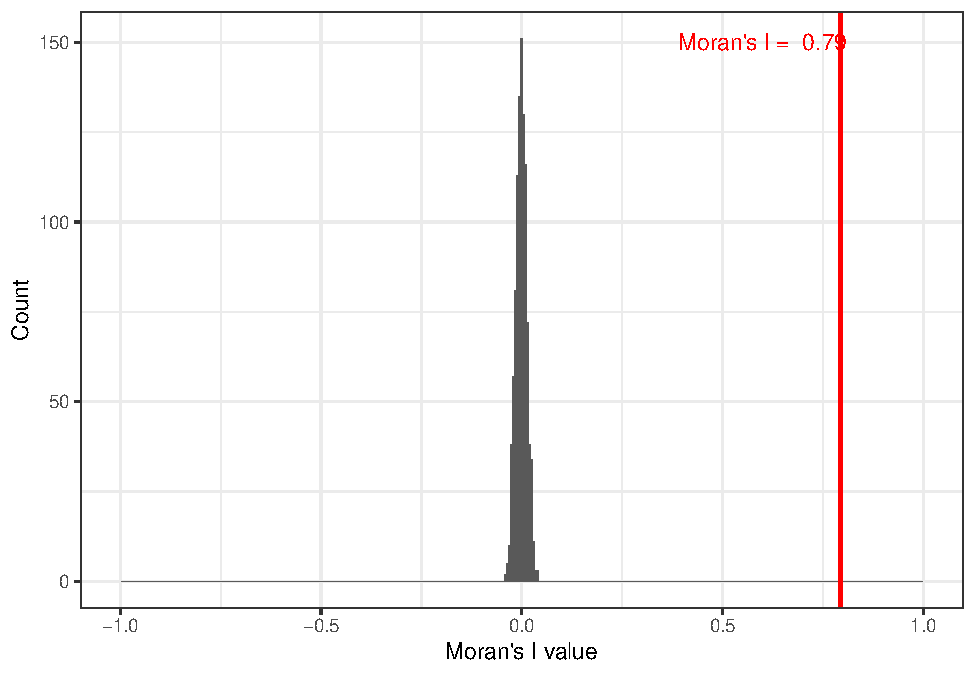
\includegraphics{HW2-SpatialRegression_files/figure-latex/unnamed-chunk-1-1.pdf}

\hypertarget{local-morans-i}{%
\subsubsection{Local Moran's I}\label{local-morans-i}}

The Local Moran's I result, presented through the Significance Map and
Cluster Map, reveal distinct patterns within the spatial distribution of
the variable of interest LNMEDHVAL. The `not significant' areas
represent regions where no significant spatial clustering or outliers
were identified, suggesting a relatively homogeneous spatial pattern. In
contrast, the `high-high' clusters indicate areas where high values
LNMEDHVAL are surrounded by other high values, signifying spatial
clusters of high values. Conversely, the `low-low' clusters represent
areas characterized by low values surrounded by other low values,
indicating spatial clusters of low values. The `high-low' areas depict
locations where high values of the variable are surrounded by
neighboring areas with low values, suggesting the presence of stark
spatial outliers. Similarly, the `low-high' areas denote regions where
low values are surrounded by neighboring areas with high values,
representing contrasting spatial outliers.

Based on the Local Moran's I result there are significant clusters of
high-high values in Center City, South Kensington, Society Hill, and
Rittenhouse Square. Significant clusters of low-low values can be found
in North Philadelphia, Kensington, Southwest Philadelphia, and Olney.
Areas of with high-low clustering include Germantown, Morrell Park, and
Normandy Village. Areas with low-high clustering include
Aston-Woodbridge, Mill Creek. Not significant areas include South
Philadelphia, Kensington, and west Philadelphia.

\begin{Shaded}
\begin{Highlighting}[]
\CommentTok{\#Run local moran\textquotesingle{}s I (LISA)}

\NormalTok{LISA}\OtherTok{\textless{}{-}}\FunctionTok{localmoran}\NormalTok{(data}\SpecialCharTok{$}\NormalTok{LNMEDHVAL, queenlist)}
\NormalTok{data\_LISA }\OtherTok{\textless{}{-}}\FunctionTok{cbind}\NormalTok{(data, }\FunctionTok{as.data.frame}\NormalTok{(LISA))}

\NormalTok{quadrant}\OtherTok{\textless{}{-}}\FunctionTok{vector}\NormalTok{(}\AttributeTok{mode=}\StringTok{\textquotesingle{}numeric\textquotesingle{}}\NormalTok{, }\AttributeTok{length=}\DecValTok{323}\NormalTok{)}
\NormalTok{m.prop}\OtherTok{\textless{}{-}}\NormalTok{data}\SpecialCharTok{$}\NormalTok{LNMEDHVAL }\SpecialCharTok{{-}} \FunctionTok{mean}\NormalTok{(data}\SpecialCharTok{$}\NormalTok{LNMEDHVAL)}
\NormalTok{m.local}\OtherTok{\textless{}{-}}\NormalTok{LISA[,}\DecValTok{1}\NormalTok{]}\SpecialCharTok{{-}}\FunctionTok{mean}\NormalTok{(LISA[,}\DecValTok{1}\NormalTok{])}
\NormalTok{quadrant[m.prop }\SpecialCharTok{\textgreater{}}\DecValTok{0} \SpecialCharTok{\&}\NormalTok{ m.local}\SpecialCharTok{\textgreater{}}\DecValTok{0}\NormalTok{]}\OtherTok{\textless{}{-}}\StringTok{\textquotesingle{}4\textquotesingle{}} \CommentTok{\#high MEDHHINC, high clustering}
\NormalTok{quadrant[m.prop }\SpecialCharTok{\textless{}}\DecValTok{0} \SpecialCharTok{\&}\NormalTok{ m.local}\SpecialCharTok{\textless{}}\DecValTok{0}\NormalTok{]}\OtherTok{\textless{}{-}}\StringTok{\textquotesingle{}1\textquotesingle{}} \CommentTok{\#low MEDHHINC, low clustering}
\NormalTok{quadrant[m.prop }\SpecialCharTok{\textless{}}\DecValTok{0} \SpecialCharTok{\&}\NormalTok{ m.local}\SpecialCharTok{\textgreater{}}\DecValTok{0}\NormalTok{]}\OtherTok{\textless{}{-}}\StringTok{\textquotesingle{}2\textquotesingle{}} \CommentTok{\#low MEDHINC, high clustering}
\NormalTok{quadrant[m.prop }\SpecialCharTok{\textgreater{}}\DecValTok{0} \SpecialCharTok{\&}\NormalTok{ m.local}\SpecialCharTok{\textless{}}\DecValTok{0}\NormalTok{]}\OtherTok{\textless{}{-}}\StringTok{\textquotesingle{}3\textquotesingle{}} \CommentTok{\#high MEDHHINC, low clustering}
\NormalTok{quadrant[LISA[,}\DecValTok{5}\NormalTok{]}\SpecialCharTok{\textgreater{}}\FloatTok{0.05}\NormalTok{]}\OtherTok{\textless{}{-}}\DecValTok{0}

\NormalTok{data\_LISA }\OtherTok{\textless{}{-}}\FunctionTok{cbind}\NormalTok{(data, }\FunctionTok{as.data.frame}\NormalTok{(LISA), }\FunctionTok{as.data.frame}\NormalTok{(quadrant))}
\end{Highlighting}
\end{Shaded}

\begin{Shaded}
\begin{Highlighting}[]
\FunctionTok{grid.arrange}\NormalTok{(}\AttributeTok{ncol=}\DecValTok{3}\NormalTok{,}
             
\FunctionTok{ggplot}\NormalTok{()}\SpecialCharTok{+}
  \FunctionTok{geom\_sf}\NormalTok{(}\AttributeTok{data=}\NormalTok{data,}\FunctionTok{aes}\NormalTok{(}\AttributeTok{fill=}\NormalTok{LNMEDHVAL))}\SpecialCharTok{+}
  \FunctionTok{scale\_fill\_viridis\_c}\NormalTok{(}\AttributeTok{option=}\StringTok{\textquotesingle{}rocket\textquotesingle{}}\NormalTok{,}\AttributeTok{direction=}\SpecialCharTok{{-}}\DecValTok{1}\NormalTok{)}\SpecialCharTok{+}
  \FunctionTok{theme\_void}\NormalTok{()}\SpecialCharTok{+}
  \FunctionTok{theme}\NormalTok{(}\AttributeTok{panel.background =} \FunctionTok{element\_rect}\NormalTok{(}\AttributeTok{fill=}\StringTok{\textquotesingle{}white\textquotesingle{}}\NormalTok{),}
        \AttributeTok{legend.position =} \FunctionTok{c}\NormalTok{(}\FloatTok{0.80}\NormalTok{, }\FloatTok{0.21}\NormalTok{),}
        \AttributeTok{plot.title =} \FunctionTok{element\_text}\NormalTok{(}\AttributeTok{hjust =} \FloatTok{0.5}\NormalTok{))}\SpecialCharTok{+}
  \FunctionTok{ggtitle}\NormalTok{(}\StringTok{"Natural Log of Median Home Value"}\NormalTok{),}

\FunctionTok{ggplot}\NormalTok{()}\SpecialCharTok{+}
  \FunctionTok{geom\_sf}\NormalTok{(}\AttributeTok{data=}\NormalTok{data\_LISA,}\FunctionTok{aes}\NormalTok{(}\AttributeTok{fill =} \FunctionTok{cut}\NormalTok{(Pr.z....E.Ii.., }\AttributeTok{breaks =} \FunctionTok{c}\NormalTok{(}\DecValTok{0}\NormalTok{,}\FloatTok{0.01}\NormalTok{,}\FloatTok{0.05}\NormalTok{,}\FloatTok{0.5}\NormalTok{,}\DecValTok{1}\NormalTok{))))}\SpecialCharTok{+}
  \FunctionTok{scale\_fill\_manual}\NormalTok{(}\AttributeTok{values =} \FunctionTok{c}\NormalTok{(}\StringTok{\textquotesingle{}\#990000\textquotesingle{}}\NormalTok{,}\StringTok{\textquotesingle{}\#ef6548\textquotesingle{}}\NormalTok{,}\StringTok{\textquotesingle{}\#fdbb84\textquotesingle{}}\NormalTok{,}\StringTok{\textquotesingle{}\#fef0d9\textquotesingle{}}\NormalTok{),}
                    \AttributeTok{labels=}\FunctionTok{c}\NormalTok{(}\StringTok{\textquotesingle{}0 {-} 0.01\textquotesingle{}}\NormalTok{,}\StringTok{\textquotesingle{}0.01 {-} 0.05\textquotesingle{}}\NormalTok{,}\StringTok{\textquotesingle{}0.05 {-} 0.5\textquotesingle{}}\NormalTok{,}\StringTok{\textquotesingle{}0.5 {-} 1\textquotesingle{}}\NormalTok{),}
                    \AttributeTok{name=}\StringTok{\textquotesingle{}p value\textquotesingle{}}\NormalTok{)}\SpecialCharTok{+}
  \FunctionTok{theme\_void}\NormalTok{()}\SpecialCharTok{+}
  \FunctionTok{theme}\NormalTok{(}\AttributeTok{panel.background =} \FunctionTok{element\_rect}\NormalTok{(}\AttributeTok{fill=}\StringTok{\textquotesingle{}white\textquotesingle{}}\NormalTok{),}
        \AttributeTok{legend.position =} \FunctionTok{c}\NormalTok{(}\FloatTok{0.80}\NormalTok{, }\FloatTok{0.21}\NormalTok{),}
        \AttributeTok{plot.title =} \FunctionTok{element\_text}\NormalTok{(}\AttributeTok{hjust =} \FloatTok{0.5}\NormalTok{))}\SpecialCharTok{+}
  \FunctionTok{ggtitle}\NormalTok{(}\StringTok{"Local Morans I (p value)"}\NormalTok{),}
             
\FunctionTok{ggplot}\NormalTok{()}\SpecialCharTok{+}
  \FunctionTok{geom\_sf}\NormalTok{(}\AttributeTok{data=}\NormalTok{data\_LISA,}\FunctionTok{aes}\NormalTok{(}\AttributeTok{fill=}\NormalTok{quadrant))}\SpecialCharTok{+}
  \FunctionTok{scale\_fill\_manual}\NormalTok{(}\AttributeTok{values=}\FunctionTok{c}\NormalTok{(}\StringTok{\textquotesingle{}grey80\textquotesingle{}}\NormalTok{,}\StringTok{\textquotesingle{}lightblue\textquotesingle{}}\NormalTok{,}\StringTok{\textquotesingle{}blue\textquotesingle{}}\NormalTok{,}\StringTok{\textquotesingle{}pink\textquotesingle{}}\NormalTok{,}\StringTok{\textquotesingle{}red\textquotesingle{}}\NormalTok{),}
                    \AttributeTok{labels=}\FunctionTok{c}\NormalTok{(}\StringTok{"Insignificant"}\NormalTok{,}\StringTok{"Low{-}High"}\NormalTok{,}\StringTok{"Low{-}Low"}\NormalTok{,}\StringTok{"High{-}Low"}\NormalTok{,}\StringTok{"High{-}High"}\NormalTok{),}
                    \AttributeTok{name=}\StringTok{\textquotesingle{}Significant Cluster\textquotesingle{}}\NormalTok{)}\SpecialCharTok{+}
  \FunctionTok{theme\_void}\NormalTok{()}\SpecialCharTok{+}
  \FunctionTok{theme}\NormalTok{(}\AttributeTok{panel.background =} \FunctionTok{element\_rect}\NormalTok{(}\AttributeTok{fill=}\StringTok{\textquotesingle{}white\textquotesingle{}}\NormalTok{),}
        \AttributeTok{legend.position =} \FunctionTok{c}\NormalTok{(}\FloatTok{0.80}\NormalTok{, }\FloatTok{0.21}\NormalTok{),}
        \AttributeTok{plot.title =} \FunctionTok{element\_text}\NormalTok{(}\AttributeTok{hjust =} \FloatTok{0.5}\NormalTok{))}\SpecialCharTok{+}
  \FunctionTok{ggtitle}\NormalTok{(}\StringTok{"Significant Clusters of High/Low Values"}\NormalTok{)}
\NormalTok{)}
\end{Highlighting}
\end{Shaded}

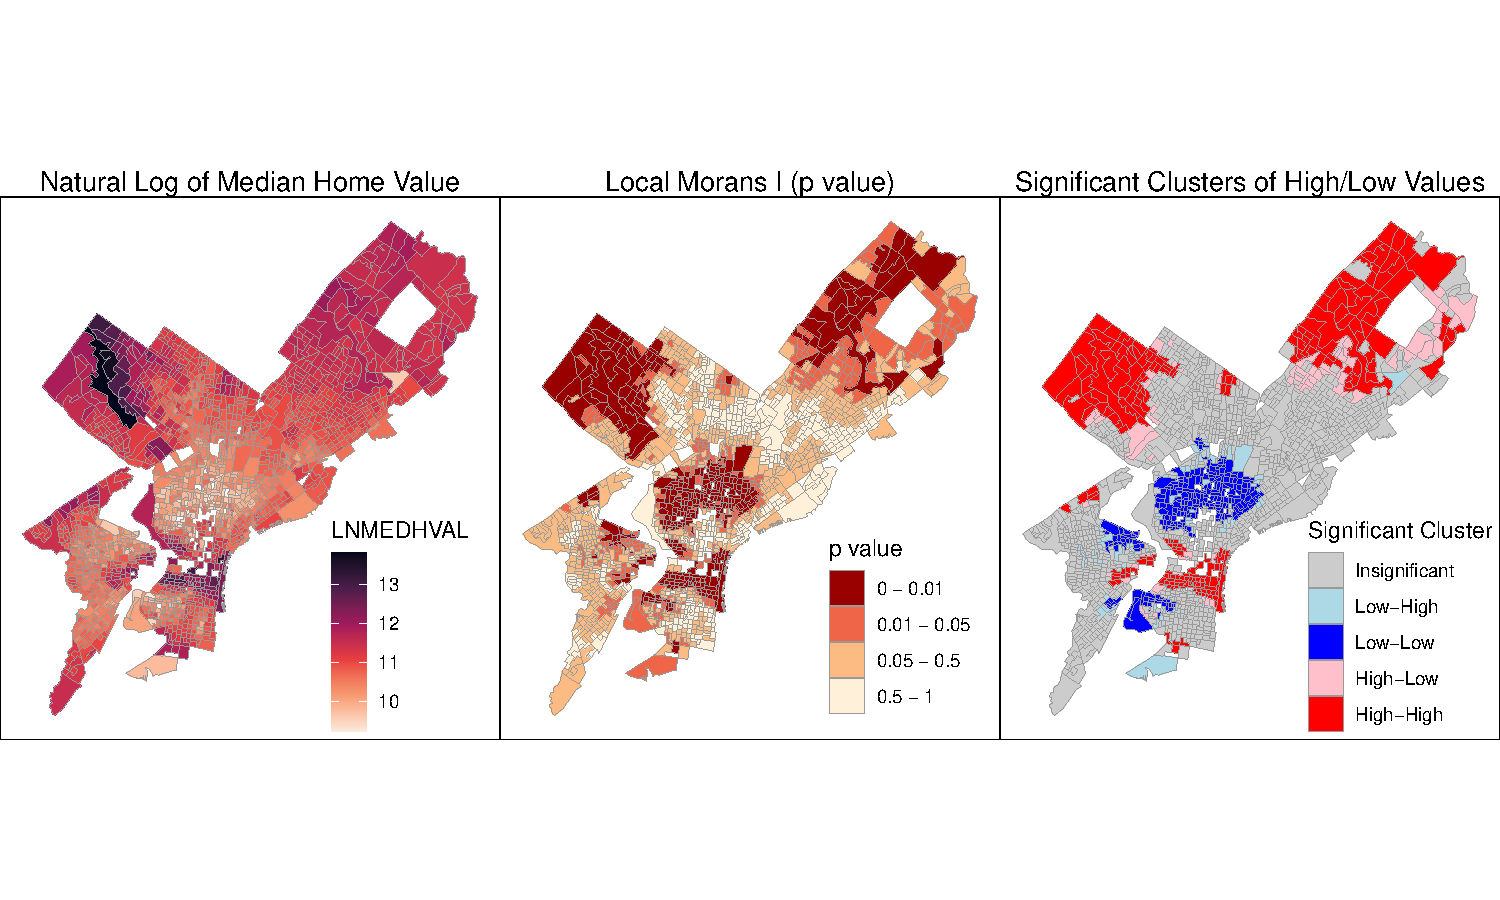
\includegraphics{HW2-SpatialRegression_files/figure-latex/Morans_I_map-1.pdf}

\hypertarget{a-review-of-ols-regression-and-assumptions-1}{%
\subsection{A Review of OLS Regression and
Assumptions:}\label{a-review-of-ols-regression-and-assumptions-1}}

\hypertarget{ols-results}{%
\subsubsection{OLS Results}\label{ols-results}}

The (OLS) regression results identified that poverty levels, education
status, home vacancy rates, and single-resident homes are statistically
significant predictors of the natural log of median home values in
Philadelphia, with an R\^{}2 value of 0.6623, explaining 66.23\% of the
variance in median home values.

\begin{Shaded}
\begin{Highlighting}[]
\NormalTok{reg }\OtherTok{\textless{}{-}}\FunctionTok{lm}\NormalTok{(LNMEDHVAL }\SpecialCharTok{\textasciitilde{}}\NormalTok{  PCTVACANT }\SpecialCharTok{+}\NormalTok{ PCTSINGLES }\SpecialCharTok{+}\NormalTok{ PCTBACHMOR }\SpecialCharTok{+}\NormalTok{ LNNBELPOV, }\AttributeTok{data=}\NormalTok{data)}

\FunctionTok{summary}\NormalTok{(reg)}
\end{Highlighting}
\end{Shaded}

\begin{verbatim}
## 
## Call:
## lm(formula = LNMEDHVAL ~ PCTVACANT + PCTSINGLES + PCTBACHMOR + 
##     LNNBELPOV, data = data)
## 
## Residuals:
##      Min       1Q   Median       3Q      Max 
## -2.25817 -0.20391  0.03822  0.21743  2.24345 
## 
## Coefficients:
##               Estimate Std. Error t value Pr(>|t|)    
## (Intercept) 11.1137781  0.0465318 238.843  < 2e-16 ***
## PCTVACANT   -0.0191563  0.0009779 -19.590  < 2e-16 ***
## PCTSINGLES   0.0029770  0.0007032   4.234 2.42e-05 ***
## PCTBACHMOR   0.0209095  0.0005432  38.494  < 2e-16 ***
## LNNBELPOV   -0.0789035  0.0084567  -9.330  < 2e-16 ***
## ---
## Signif. codes:  0 '***' 0.001 '**' 0.01 '*' 0.05 '.' 0.1 ' ' 1
## 
## Residual standard error: 0.3665 on 1715 degrees of freedom
## Multiple R-squared:  0.6623, Adjusted R-squared:  0.6615 
## F-statistic: 840.9 on 4 and 1715 DF,  p-value: < 2.2e-16
\end{verbatim}

\hypertarget{heteroscedasticity-tests}{%
\subsubsection{Heteroscedasticity
tests}\label{heteroscedasticity-tests}}

The results from the Breusch-Pagan, Koenker-Bassett, and White's tests
for heteroscedasticity are consistent with one another, each providing
strong evidence against the null hypothesis of homoscedasticity in the
regression model. All the test's p-values suggest that the variance of
the residuals is not constant across observations, with p-values
significantly below the common alpha level of 0.05, which in this case
are less than 2.2e-16 (Breusch-Pagan) and 1.102e-08, respectively. The
Koenker-Bassett test produces a high-test statistic of 43.94 which
suggests strong evidence of heteroskedasticity. These very low p-values
and high test statistic lead to the rejection of the null hypothesis of
homoscedasticity of the models residuals ( i.e., having a constant
variance).

\begin{Shaded}
\begin{Highlighting}[]
\CommentTok{\#Prints the results of the Breusch{-}Pagan Test to assess whether heteroscedasticity is present (package: lmtest)}
\FunctionTok{bptest}\NormalTok{(reg, }\AttributeTok{studentize=}\ConstantTok{FALSE}\NormalTok{)}
\end{Highlighting}
\end{Shaded}

\begin{verbatim}
## 
##  Breusch-Pagan test
## 
## data:  reg
## BP = 113.19, df = 4, p-value < 2.2e-16
\end{verbatim}

\begin{Shaded}
\begin{Highlighting}[]
\CommentTok{\#Prints the results of the Koenker{-}Bassett Test (also known as the Studentized Breusch{-}Pagan Test) to assess whether heteroscedasticity is present (package: lmtest)}
\FunctionTok{bptest}\NormalTok{(reg)      }
\end{Highlighting}
\end{Shaded}

\begin{verbatim}
## 
##  studentized Breusch-Pagan test
## 
## data:  reg
## BP = 42.868, df = 4, p-value = 1.102e-08
\end{verbatim}

\begin{Shaded}
\begin{Highlighting}[]
\CommentTok{\#Prints the results of the White Test to assess whether heteroscedasticity is present (package: whitestrap)}
\FunctionTok{white\_test}\NormalTok{(reg)}
\end{Highlighting}
\end{Shaded}

\begin{verbatim}
## White's test results
## 
## Null hypothesis: Homoskedasticity of the residuals
## Alternative hypothesis: Heteroskedasticity of the residuals
## Test Statistic: 43.94
## P-value: 0
\end{verbatim}

\begin{Shaded}
\begin{Highlighting}[]
\NormalTok{data }\OtherTok{\textless{}{-}}\NormalTok{ data }\SpecialCharTok{\%\textgreater{}\%}
  \FunctionTok{mutate}\NormalTok{(}\AttributeTok{predictions =} \FunctionTok{predict}\NormalTok{(reg,data),}
        \AttributeTok{residual =}\NormalTok{ LNMEDHVAL }\SpecialCharTok{{-}}\NormalTok{ predictions,}
        \AttributeTok{stdres =} \FunctionTok{rstandard}\NormalTok{(reg))}

\FunctionTok{ggplot}\NormalTok{()}\SpecialCharTok{+}
  \FunctionTok{geom\_point}\NormalTok{(}\AttributeTok{data=}\NormalTok{data,}\FunctionTok{aes}\NormalTok{(}\AttributeTok{x=}\NormalTok{predictions,}\AttributeTok{y=}\NormalTok{stdres),}\AttributeTok{size=}\FloatTok{0.4}
\NormalTok{            )}\SpecialCharTok{+}
  \FunctionTok{labs}\NormalTok{(}\AttributeTok{x=}\StringTok{\textquotesingle{}Predicted Values\textquotesingle{}}\NormalTok{,}\AttributeTok{y=}\StringTok{\textquotesingle{}Standardized Residuals\textquotesingle{}}\NormalTok{)}\SpecialCharTok{+}
  \FunctionTok{ggtitle}\NormalTok{(}\StringTok{\textquotesingle{}Predicted Values vs. Standardized Residuals\textquotesingle{}}\NormalTok{)}\SpecialCharTok{+}
  \FunctionTok{theme\_bw}\NormalTok{()}
\end{Highlighting}
\end{Shaded}

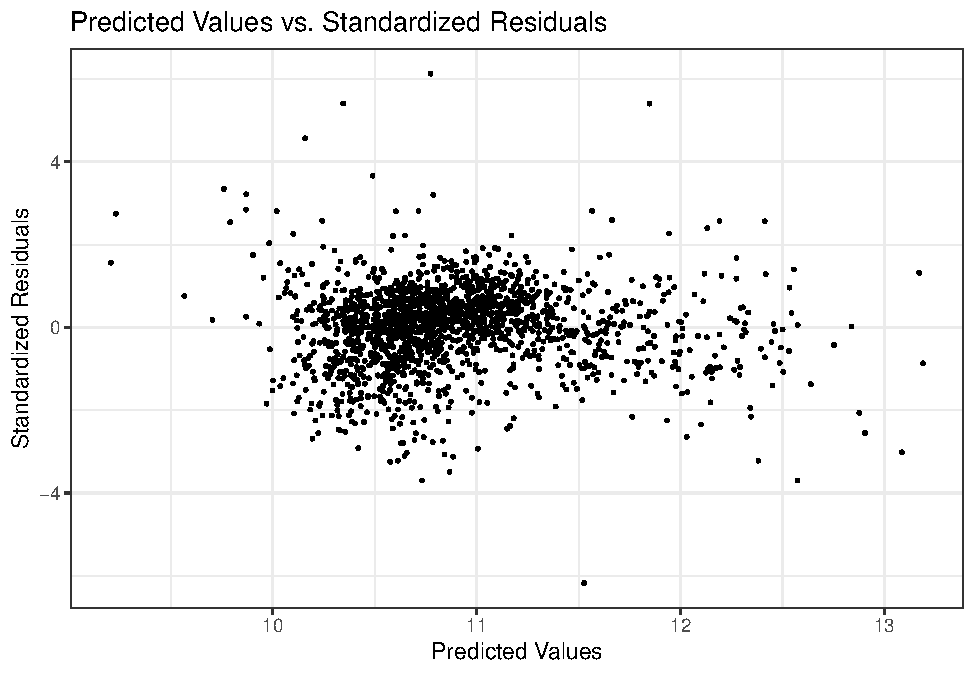
\includegraphics{HW2-SpatialRegression_files/figure-latex/scatter_plot-1.pdf}

The conclusion from the Breusch-Pagan, Koenker-Bassett, and White's
tests for heteroscedasticity is consistent with the observations made
from the residual by predicted plot presented in to ``Assignment 1 --
OLS Regression''. The ``bow-tie'' shape observed in the scatter plot
around the predicted value of 11.5 is a visual indication of
heteroscedasticity, where the spread of residuals increases at certain
levels of the predicted variable, deviating from what would be expected
in a homoscedastic relationship. This analysis complements the
statistical evidence provided by the tests, which also suggests
non-constant variance in the residuals.

\hypertarget{normality-of-errors-jarque-bera-test}{%
\subsubsection{Normality of errors (Jarque-Bera
test)}\label{normality-of-errors-jarque-bera-test}}

According to the Jarque-Bera test results, the assumption of normality
for the regression errors is violated. The provided p-value is less than
2.2e-16, which is far below the conventional significance level
(p\textless{} 0.05). This extremely low p-value leads to the rejection
of the null hypothesis that the residuals are normally distributed.
These results are not consistent with the histogram of residuals
presented in ``Assignment 1 -- OLS Regression''. This inconsistency can
be attributed to the limits and accuracy of visual interpretation of
histogram results. While the histogram of the residuals suggests a
roughly normal distribution at a glance, the Jarque-Bera test is a
nuanced tool that captures subtle deviations in skewness that are not
immediately evident in the visual representation.

\begin{Shaded}
\begin{Highlighting}[]
\CommentTok{\#Prints the results of the Jarque{-}Bera Test to assess whether residuals are normal (package: tseries)}
\FunctionTok{jarque.bera.test}\NormalTok{(data}\SpecialCharTok{$}\NormalTok{residual)}
\end{Highlighting}
\end{Shaded}

\begin{verbatim}
## 
##  Jarque Bera Test
## 
## data:  data$residual
## X-squared = 778.96, df = 2, p-value < 2.2e-16
\end{verbatim}

\begin{Shaded}
\begin{Highlighting}[]
\FunctionTok{ggplot}\NormalTok{()}\SpecialCharTok{+}
  \FunctionTok{geom\_histogram}\NormalTok{(}\AttributeTok{data=}\NormalTok{data,}\FunctionTok{aes}\NormalTok{(}\AttributeTok{x=}\NormalTok{stdres),}\AttributeTok{bins=}\DecValTok{100}\NormalTok{,}\AttributeTok{color=}\StringTok{\textquotesingle{}white\textquotesingle{}}\NormalTok{,}\AttributeTok{fill=}\StringTok{\textquotesingle{}grey50\textquotesingle{}}\NormalTok{)}\SpecialCharTok{+}
  \FunctionTok{labs}\NormalTok{(}\AttributeTok{x=}\StringTok{\textquotesingle{}Standardized residual\textquotesingle{}}\NormalTok{)}\SpecialCharTok{+}
  \FunctionTok{theme\_bw}\NormalTok{()}
\end{Highlighting}
\end{Shaded}

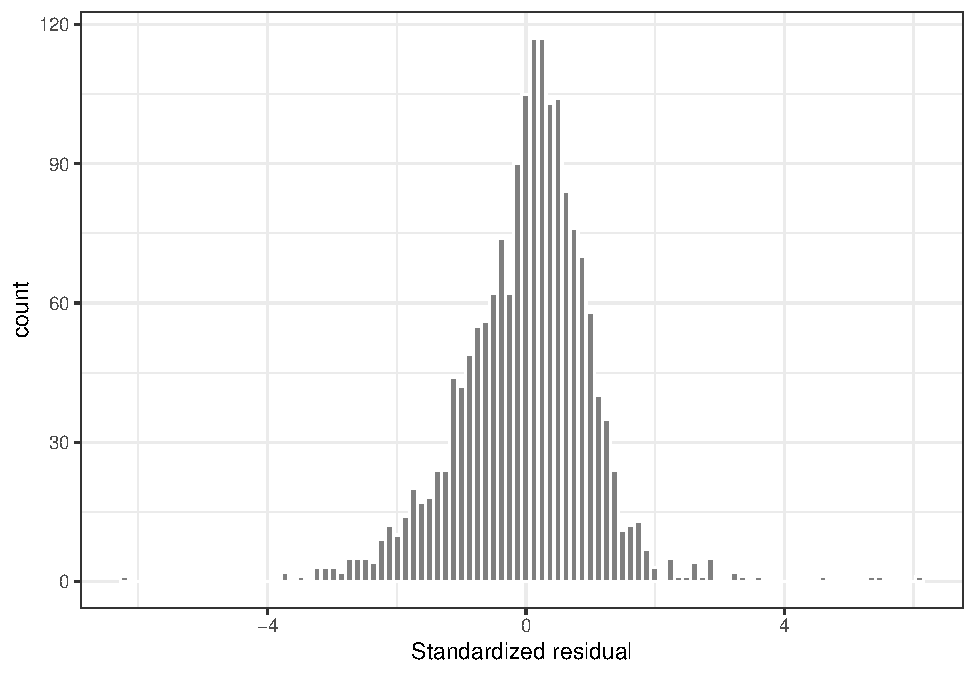
\includegraphics{HW2-SpatialRegression_files/figure-latex/histogram-1.pdf}

\hypertarget{morans-i-plot}{%
\subsubsection{Morans I plot}\label{morans-i-plot}}

By regressing the standardized residuals on the spatially lagged
residuals we can see that that the beta coefficient (slope b) of the of
the lagged residual is 0.312. Meaning, that as the lagged residual
changes by 1 unit, the standardized residual changes by 0.312 units.
This is a key indicator of spatial autocorrelation, which suggests that
nearby or neighboring residuals are similar. When this coefficient is
significantly different from zero, it means that there's a statistically
significant spatial autocorrelation in the residuals of the model

\begin{Shaded}
\begin{Highlighting}[]
\NormalTok{data}\SpecialCharTok{$}\NormalTok{resnb}\OtherTok{\textless{}{-}}\FunctionTok{sapply}\NormalTok{(queen, }\ControlFlowTok{function}\NormalTok{(x) }\FunctionTok{mean}\NormalTok{(data}\SpecialCharTok{$}\NormalTok{stdres[x]))}

\NormalTok{res.lm }\OtherTok{\textless{}{-}} \FunctionTok{lm}\NormalTok{(}\AttributeTok{formula=}\NormalTok{data}\SpecialCharTok{$}\NormalTok{resnb }\SpecialCharTok{\textasciitilde{}}\NormalTok{ data}\SpecialCharTok{$}\NormalTok{stdres)}

\CommentTok{\#This code is all to get the p{-}value and beta coefficient from the regression summary so that we can annotate thoose values on the scatter plot. It might not be necessary and we can just show the regression summary in addition to the scatter plot. I added it because the GeoDa results include an annotation with the coefficient.}

\NormalTok{p\_value }\OtherTok{\textless{}{-}} \FunctionTok{summary}\NormalTok{(res.lm)}\SpecialCharTok{$}\NormalTok{coefficients[}\DecValTok{2}\NormalTok{,}\DecValTok{4}\NormalTok{]}
\NormalTok{coefficient}\OtherTok{=} \FunctionTok{summary}\NormalTok{(res.lm)}\SpecialCharTok{$}\NormalTok{coefficients[}\DecValTok{2}\NormalTok{,}\DecValTok{1}\NormalTok{]}
\NormalTok{p\_value }\OtherTok{=} \FunctionTok{format}\NormalTok{(p\_value, }\AttributeTok{scientific =} \ConstantTok{TRUE}\NormalTok{)}

\FunctionTok{ggplot}\NormalTok{(}\AttributeTok{data=}\NormalTok{data,}\FunctionTok{aes}\NormalTok{(}\AttributeTok{x=}\NormalTok{stdres,}\AttributeTok{y=}\NormalTok{resnb))}\SpecialCharTok{+}
  \FunctionTok{geom\_point}\NormalTok{(}\AttributeTok{size=}\FloatTok{0.4}\NormalTok{)}\SpecialCharTok{+}
  \FunctionTok{geom\_smooth}\NormalTok{(}\AttributeTok{method =} \StringTok{"lm"}\NormalTok{, }\AttributeTok{se =} \ConstantTok{FALSE}\NormalTok{,}\AttributeTok{color=}\StringTok{\textquotesingle{}blue\textquotesingle{}}\NormalTok{,}\AttributeTok{linewidth=}\FloatTok{0.5}\NormalTok{)}\SpecialCharTok{+}
  \FunctionTok{annotate}\NormalTok{(}\StringTok{"text"}\NormalTok{,}\AttributeTok{x=}\DecValTok{4}\NormalTok{, }\AttributeTok{y=}\SpecialCharTok{{-}}\DecValTok{2}\NormalTok{,}\AttributeTok{color=}\StringTok{\textquotesingle{}red\textquotesingle{}}\NormalTok{,}\AttributeTok{label=}\FunctionTok{paste}\NormalTok{(}\StringTok{"Coefficient: "}\NormalTok{,}\FunctionTok{as.character}\NormalTok{(}\FunctionTok{round}\NormalTok{(coefficient,}\DecValTok{3}\NormalTok{))))}\SpecialCharTok{+}
  \FunctionTok{annotate}\NormalTok{(}\StringTok{"text"}\NormalTok{,}\AttributeTok{x=}\DecValTok{4}\NormalTok{, }\AttributeTok{y=}\SpecialCharTok{{-}}\FloatTok{2.3}\NormalTok{,}\AttributeTok{color=}\StringTok{\textquotesingle{}red\textquotesingle{}}\NormalTok{,}\AttributeTok{label=}\FunctionTok{paste}\NormalTok{(}\StringTok{"p{-}value: "}\NormalTok{,}\FunctionTok{as.character}\NormalTok{((p\_value))))}\SpecialCharTok{+}
  \FunctionTok{labs}\NormalTok{(}\AttributeTok{x=}\StringTok{\textquotesingle{}Standardized Residuals\textquotesingle{}}\NormalTok{,}\AttributeTok{y=}\StringTok{\textquotesingle{}Spatially Lagged Standardized Residuals\textquotesingle{}}\NormalTok{)}\SpecialCharTok{+}
  \FunctionTok{ggtitle}\NormalTok{(}\StringTok{\textquotesingle{}Standardized Resiudals vs Lagged Standardized Residuals\textquotesingle{}}\NormalTok{)}\SpecialCharTok{+}
  \FunctionTok{theme\_bw}\NormalTok{()}
\end{Highlighting}
\end{Shaded}

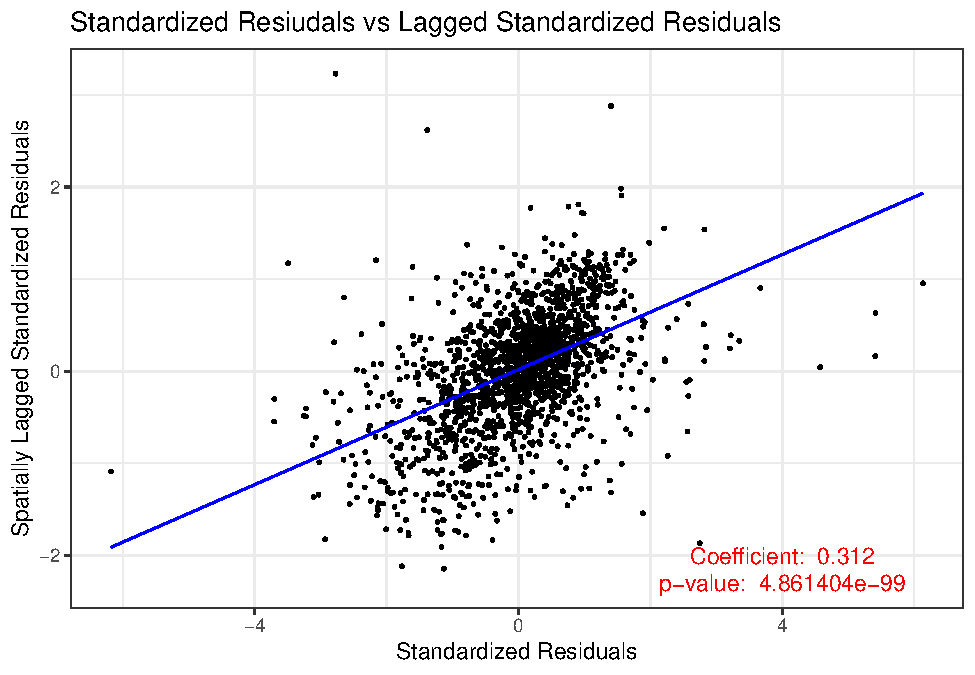
\includegraphics{HW2-SpatialRegression_files/figure-latex/unnamed-chunk-2-1.pdf}

\hypertarget{morans-i-permutation-results}{%
\subsubsection{Morans I Permutation
Results}\label{morans-i-permutation-results}}

The observed Moran's I value of 0.31, significantly distanced from the
permutation distribution's center, which reveals substantial spatial
autocorrelation in the OLS residuals. This is problematic because it
violates the assumption that the residuals are independently
distributed. Both Moran's I and the beta coefficient of the spatially
lagged residuals tell a similar story in that they both indicate the
presence of spatial autocorrelation. The beta coefficient quantifies the
relationship between the residuals and their spatial lags, while Moran's
I provides an overall measure of spatial autocorrelation. The results of
both statistics indicating positive spatial autocorrelation reinforce
the conclusion that the OLS model's residuals are not independent and
that there is a pattern to their spatial distribution.

\begin{Shaded}
\begin{Highlighting}[]
\NormalTok{moranMC\_OLSres}\OtherTok{\textless{}{-}}\FunctionTok{moran.mc}\NormalTok{(data}\SpecialCharTok{$}\NormalTok{stdres, queenlist, }\AttributeTok{nsim=}\DecValTok{999}\NormalTok{, }\AttributeTok{alternative=}\StringTok{"two.sided"}\NormalTok{)  }\CommentTok{\#We use 999 permutations}

\CommentTok{\#Draws distribution of Moran\textquotesingle{}s I\textquotesingle{}s calculated from randomly permuted values}
\CommentTok{\# Here, we draw a red vertical line at the observed value of our Moran\textquotesingle{}s I}

\FunctionTok{ggplot}\NormalTok{()}\SpecialCharTok{+}
  \FunctionTok{geom\_histogram}\NormalTok{(}\FunctionTok{aes}\NormalTok{(moranMC\_OLSres}\SpecialCharTok{$}\NormalTok{res),}\AttributeTok{binwidth =} \FloatTok{0.005}\NormalTok{)}\SpecialCharTok{+}
  \FunctionTok{xlim}\NormalTok{(}\SpecialCharTok{{-}}\DecValTok{1}\NormalTok{,}\DecValTok{1}\NormalTok{)}\SpecialCharTok{+}
  \FunctionTok{geom\_vline}\NormalTok{(}\AttributeTok{xintercept=}\NormalTok{moranMC\_OLSres}\SpecialCharTok{$}\NormalTok{statistic,}\AttributeTok{color=}\StringTok{\textquotesingle{}red\textquotesingle{}}\NormalTok{,}\AttributeTok{linewidth=}\DecValTok{1}\NormalTok{)}\SpecialCharTok{+}
  \FunctionTok{annotate}\NormalTok{(}\StringTok{"text"}\NormalTok{,}\AttributeTok{x=}\FloatTok{0.6}\NormalTok{, }\AttributeTok{y=}\DecValTok{150}\NormalTok{,}\AttributeTok{color=}\StringTok{\textquotesingle{}red\textquotesingle{}}\NormalTok{,}\AttributeTok{label=}\FunctionTok{paste}\NormalTok{(}\StringTok{"Moran\textquotesingle{}s I = "}\NormalTok{,}\FunctionTok{as.character}\NormalTok{(}\FunctionTok{round}\NormalTok{(moranMC\_OLSres}\SpecialCharTok{$}\NormalTok{statistic,}\DecValTok{2}\NormalTok{))))}\SpecialCharTok{+}
  \FunctionTok{labs}\NormalTok{(}\AttributeTok{x=}\StringTok{"Moran\textquotesingle{}s I value"}\NormalTok{,}\AttributeTok{y=}\StringTok{\textquotesingle{}Count\textquotesingle{}}\NormalTok{)}\SpecialCharTok{+}
  \FunctionTok{theme\_bw}\NormalTok{()}
\end{Highlighting}
\end{Shaded}

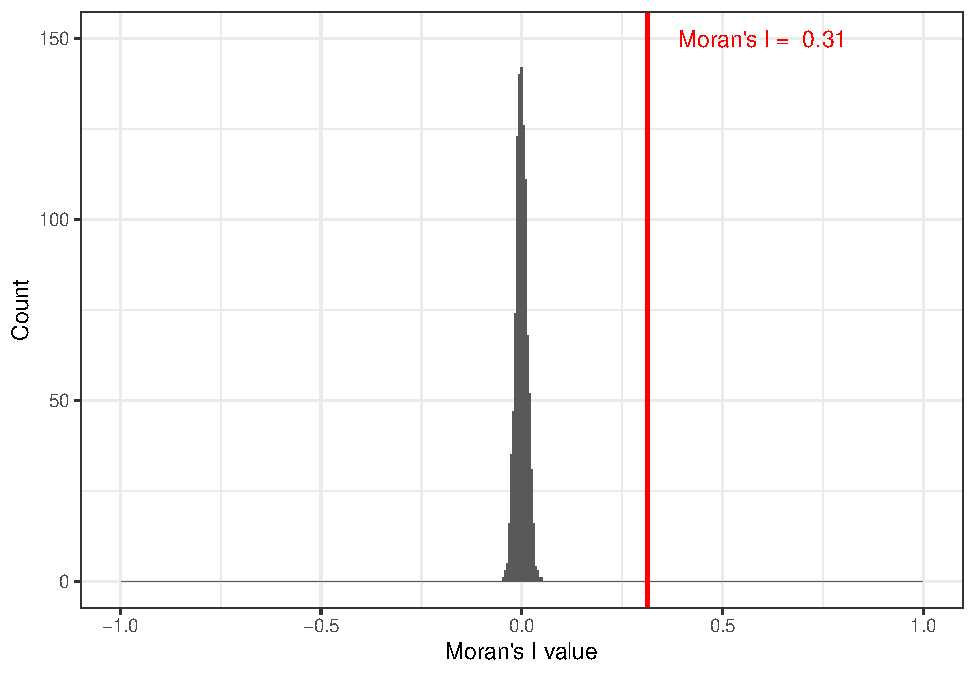
\includegraphics{HW2-SpatialRegression_files/figure-latex/unnamed-chunk-3-1.pdf}

\hypertarget{spatial-lag-and-spatial-error-regressions}{%
\subsection{Spatial Lag and Spatial Error
Regressions}\label{spatial-lag-and-spatial-error-regressions}}

\hypertarget{spatial-lag-regression}{%
\subsubsection{Spatial Lag Regression}\label{spatial-lag-regression}}

\begin{Shaded}
\begin{Highlighting}[]
\NormalTok{lagreg}\OtherTok{\textless{}{-}}\FunctionTok{lagsarlm}\NormalTok{(}\AttributeTok{formula=}\NormalTok{LNMEDHVAL }\SpecialCharTok{\textasciitilde{}}\NormalTok{ LNNBELPOV }\SpecialCharTok{+}\NormalTok{ PCTBACHMOR }\SpecialCharTok{+}\NormalTok{ PCTSINGLES }\SpecialCharTok{+}\NormalTok{ PCTVACANT, }\AttributeTok{data=}\NormalTok{data, queenlist)}
\FunctionTok{summary}\NormalTok{(lagreg)}
\end{Highlighting}
\end{Shaded}

\begin{verbatim}
## 
## Call:lagsarlm(formula = LNMEDHVAL ~ LNNBELPOV + PCTBACHMOR + PCTSINGLES + 
##     PCTVACANT, data = data, listw = queenlist)
## 
## Residuals:
##       Min        1Q    Median        3Q       Max 
## -1.655421 -0.117248  0.018654  0.133126  1.726436 
## 
## Type: lag 
## Coefficients: (asymptotic standard errors) 
##                Estimate  Std. Error  z value  Pr(>|z|)
## (Intercept)  3.89845505  0.20111357  19.3843 < 2.2e-16
## LNNBELPOV   -0.03405466  0.00629287  -5.4116 6.246e-08
## PCTBACHMOR   0.00851381  0.00052193  16.3120 < 2.2e-16
## PCTSINGLES   0.00203342  0.00051577   3.9425 8.064e-05
## PCTVACANT   -0.00852940  0.00074367 -11.4694 < 2.2e-16
## 
## Rho: 0.6511, LR test value: 911.51, p-value: < 2.22e-16
## Asymptotic standard error: 0.01805
##     z-value: 36.072, p-value: < 2.22e-16
## Wald statistic: 1301.2, p-value: < 2.22e-16
## 
## Log likelihood: -255.74 for lag model
## ML residual variance (sigma squared): 0.071948, (sigma: 0.26823)
## Number of observations: 1720 
## Number of parameters estimated: 7 
## AIC: 525.48, (AIC for lm: 1435)
## LM test for residual autocorrelation
## test value: 67.737, p-value: 2.2204e-16
\end{verbatim}

\begin{Shaded}
\begin{Highlighting}[]
\FunctionTok{LR.Sarlm}\NormalTok{(lagreg, reg) }\CommentTok{\#Here lagreg is the SL output; reg is the OLS output}
\end{Highlighting}
\end{Shaded}

\begin{verbatim}
## 
##  Likelihood ratio for spatial linear models
## 
## data:  
## Likelihood ratio = 911.51, df = 1, p-value < 2.2e-16
## sample estimates:
## Log likelihood of lagreg    Log likelihood of reg 
##                -255.7400                -711.4933
\end{verbatim}

\begin{Shaded}
\begin{Highlighting}[]
\CommentTok{\#Prints the results of the Breusch{-}Pagan Test to assess whether heteroscedasticity is present (package: lmtest)}
\FunctionTok{bptest.Sarlm}\NormalTok{(lagreg, }\AttributeTok{studentize=}\ConstantTok{FALSE}\NormalTok{)}
\end{Highlighting}
\end{Shaded}

\begin{verbatim}
## 
##  Breusch-Pagan test
## 
## data:  
## BP = 210.76, df = 4, p-value < 2.2e-16
\end{verbatim}

\begin{Shaded}
\begin{Highlighting}[]
\CommentTok{\#Prints the results of the Koenker{-}Bassett Test (also known as the Studentized Breusch{-}Pagan Test) to assess whether heteroscedasticity is present (package: lmtest)}
\FunctionTok{bptest.Sarlm}\NormalTok{(lagreg)     }
\end{Highlighting}
\end{Shaded}

\begin{verbatim}
## 
##  studentized Breusch-Pagan test
## 
## data:  
## BP = 51.411, df = 4, p-value = 1.832e-10
\end{verbatim}

\begin{Shaded}
\begin{Highlighting}[]
\CommentTok{\#Prints the results of the Jarque{-}Bera Test to assess whether residuals are normal (package: tseries)}
\FunctionTok{jarque.bera.test}\NormalTok{(lagreg}\SpecialCharTok{$}\NormalTok{residuals)}
\end{Highlighting}
\end{Shaded}

\begin{verbatim}
## 
##  Jarque Bera Test
## 
## data:  lagreg$residuals
## X-squared = 2756.9, df = 2, p-value < 2.2e-16
\end{verbatim}

The spatial lag regression model includes a separate line of results
that provide the rho value of 0.65 and the p-value for this spatial lag
term. Our p-value is close to 0, which means our spatial lag term is
significant - as a result, we can say that median home values in an area
are associated with nearby median home values. Our other independent
variables (LNNBELPOV, PCTBACHMOR, PCTSINGLES, PCTVACANT) all have
probabilities near 0, meaning that they remain significant predictors
for median home values in an area similar to the OLS model. The
intercept value in the spatial lag model is nearly a third of the value
in the OLS model, with the coefficients becoming slightly lower for
LNNBELPOV, PCTBACHMOR, and PCTSINGLES and slightly higher for PCTVACANT.
The spatial lag model's Breusch-Pagan test results show a p-value near
0. Given that this p-value is less than 0.05, we conclude that the
spatial lag regression residuals are still heteroscedastic in our model.
We also compare the AIC/SC, log likelihood, and likelihood ratio test
values between our OLS regression model and spatial lag model to
determine which model is a better fit for our data:

\begin{itemize}
\tightlist
\item
  The AIC value is 525 for the spatial lag model which is significantly
  lower than the AIC of 1435 for the OLS model, indicating that the
  spatial lag model is a better fit based on that metric since it is
  lower.
\item
  The log likelihood value of the spatial lag model is -256 which is
  higher than the log likelihood value of the OLS model at -711,
  indicating that the spatial lag model is also a better fit based on
  that metric since it is higher.
\item
  The p-value for the likelihood ratio test is near 0, so we reject the
  null hypothesis that the spatial lag model is not a better fit than
  the OLS model. As a result, the spatial lag model is a better fit for
  the data than the OLS model based on the likelihood ratio test.
  \#\#\#\# Spatial Lag Moran's I Results
\end{itemize}

\begin{Shaded}
\begin{Highlighting}[]
\NormalTok{reslag}\OtherTok{\textless{}{-}}\NormalTok{lagreg}\SpecialCharTok{$}\NormalTok{residuals}
\NormalTok{lagMoranMc}\OtherTok{\textless{}{-}}\FunctionTok{moran.mc}\NormalTok{(reslag, queenlist,}\DecValTok{999}\NormalTok{, }\AttributeTok{alternative=}\StringTok{"two.sided"}\NormalTok{)}

\FunctionTok{ggplot}\NormalTok{()}\SpecialCharTok{+}
  \FunctionTok{geom\_histogram}\NormalTok{(}\FunctionTok{aes}\NormalTok{(lagMoranMc}\SpecialCharTok{$}\NormalTok{res),}\AttributeTok{binwidth =} \FloatTok{0.005}\NormalTok{)}\SpecialCharTok{+}
  \FunctionTok{xlim}\NormalTok{(}\SpecialCharTok{{-}}\DecValTok{1}\NormalTok{,}\DecValTok{1}\NormalTok{)}\SpecialCharTok{+}
  \FunctionTok{geom\_vline}\NormalTok{(}\AttributeTok{xintercept=}\NormalTok{lagMoranMc}\SpecialCharTok{$}\NormalTok{statistic,}\AttributeTok{color=}\StringTok{\textquotesingle{}red\textquotesingle{}}\NormalTok{,}\AttributeTok{linewidth=}\DecValTok{1}\NormalTok{)}\SpecialCharTok{+}
  \FunctionTok{annotate}\NormalTok{(}\StringTok{"text"}\NormalTok{,}\AttributeTok{x=}\FloatTok{0.6}\NormalTok{, }\AttributeTok{y=}\DecValTok{150}\NormalTok{,}\AttributeTok{color=}\StringTok{\textquotesingle{}red\textquotesingle{}}\NormalTok{,}\AttributeTok{label=}\FunctionTok{paste}\NormalTok{(}\StringTok{"Moran\textquotesingle{}s I = "}\NormalTok{,}\FunctionTok{as.character}\NormalTok{(}\FunctionTok{round}\NormalTok{(lagMoranMc}\SpecialCharTok{$}\NormalTok{statistic,}\DecValTok{2}\NormalTok{))))}\SpecialCharTok{+}
  \FunctionTok{labs}\NormalTok{(}\AttributeTok{x=}\StringTok{"Moran\textquotesingle{}s I value"}\NormalTok{,}\AttributeTok{y=}\StringTok{\textquotesingle{}Count\textquotesingle{}}\NormalTok{)}\SpecialCharTok{+}
  \FunctionTok{theme\_bw}\NormalTok{()}
\end{Highlighting}
\end{Shaded}

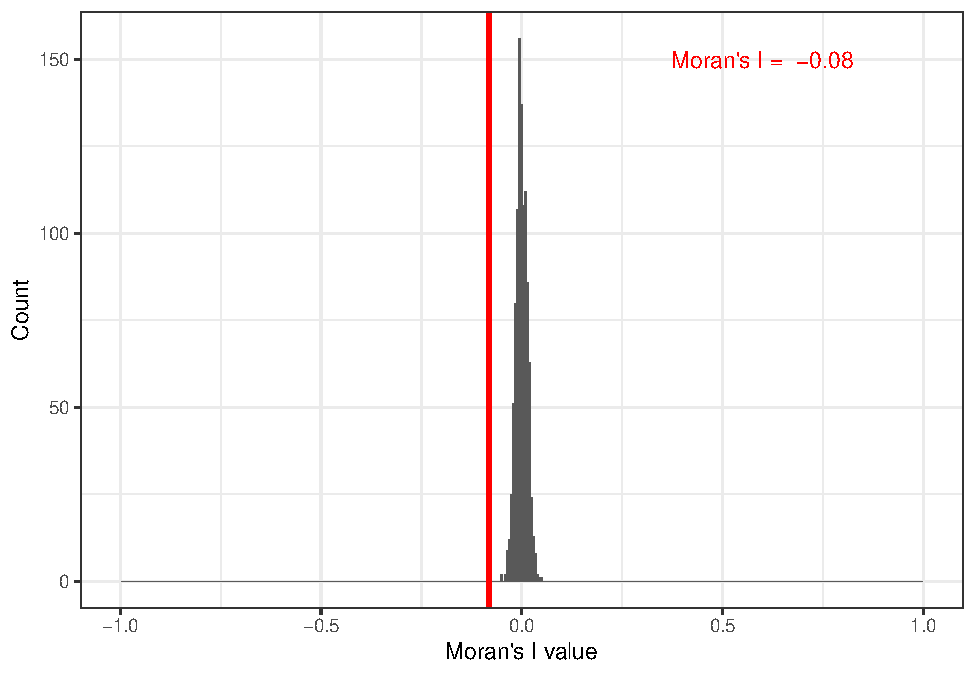
\includegraphics{HW2-SpatialRegression_files/figure-latex/unnamed-chunk-5-1.pdf}
The Moran's I value of the spatial lag model is -0.08, which is an
improvement over the Moran's I value of the OLS model at 0.31. The
spatial lag model better accounts for spatial autocorrelation in the
data and shows less spatial autocorrelation in the residuals compared to
the OLS model. Our comparison criteria show that the spatial lag model
appears to better account for spatial autocorrelation in our data
compared to the OLS model. The spatial lag model has a lower AIC value,
higher log likelihood value, statistically significant likelihood ratio
test, and lower Moran's I value. However, the Breusch-Pagan test shows
that there is still heteroscedasticity present in the model's residuals.
\#\#\# Spatial Error Regression The spatial error regression model
includes a separate line of results that provide the lambda value of
0.81 and the p-value for this spatial error term. Our p-value is close
to 0, which means our spatial error term is significant - as a result,
we can say that the residuals of median home values in an area are
associated with the residuals of nearby median home values. Our other
independent variables (LNNBELPOV, PCTBACHMOR, PCTSINGLES, PCTVACANT) all
have probabilities near 0, meaning that they remain significant
predictors for median home values in an area similar to the OLS model.
The intercept value in the spatial lag model is similar to the value in
the OLS model, with the coefficients becoming slightly lower for
PCTBACHMOR and PCTSINGLES and slightly higher for LNNBELPOV and
PCTVACANT. The spatial error model's Breusch-Pagan test results show a
p-value of 0.0001. Given that this p-value is less than 0.05, we
conclude that the spatial error regression residuals are still
heteroscedastic in our model. We also compare the AIC/SC, log
likelihood, and likelihood ratio test values between our OLS regression
model and spatial error model to determine which model is a better fit
for our data:

\begin{itemize}
\tightlist
\item
  The AIC value is 755 for the spatial lag model which is significantly
  lower than the AIC of 1435 for the OLS model, indicating that the
  spatial lag model is a better fit based on that metric since it is
  lower.
\item
  The log likelihood value of the spatial error model is -373 which is
  higher than the log likelihood value of the OLS model at -711,
  indicating that the spatial error model is also a better fit based on
  that metric since it is higher.
\item
  The p-value for the likelihood ratio test is near 0, so we reject the
  null hypothesis that the spatial error model is not a better fit than
  the OLS model. As a result, the spatial error model is a better fit
  for the data than the OLS model based on the likelihood ratio test.
\end{itemize}

\begin{Shaded}
\begin{Highlighting}[]
\NormalTok{errreg}\OtherTok{\textless{}{-}}\FunctionTok{errorsarlm}\NormalTok{(}\AttributeTok{formula=}\NormalTok{LNMEDHVAL }\SpecialCharTok{\textasciitilde{}}\NormalTok{ LNNBELPOV }\SpecialCharTok{+}\NormalTok{ PCTBACHMOR }\SpecialCharTok{+}\NormalTok{ PCTSINGLES }\SpecialCharTok{+}\NormalTok{ PCTVACANT, }\AttributeTok{data=}\NormalTok{data, queenlist)}
\NormalTok{reserr}\OtherTok{\textless{}{-}}\FunctionTok{residuals}\NormalTok{(errreg)}
\NormalTok{errresnb}\OtherTok{\textless{}{-}}\FunctionTok{sapply}\NormalTok{(queen, }\ControlFlowTok{function}\NormalTok{(x) }\FunctionTok{mean}\NormalTok{(reserr[x]))}
\FunctionTok{summary}\NormalTok{(errreg)}
\end{Highlighting}
\end{Shaded}

\begin{verbatim}
## 
## Call:errorsarlm(formula = LNMEDHVAL ~ LNNBELPOV + PCTBACHMOR + PCTSINGLES + 
##     PCTVACANT, data = data, listw = queenlist)
## 
## Residuals:
##       Min        1Q    Median        3Q       Max 
## -1.926477 -0.115408  0.014889  0.133852  1.948664 
## 
## Type: error 
## Coefficients: (asymptotic standard errors) 
##                Estimate  Std. Error  z value  Pr(>|z|)
## (Intercept) 10.90643423  0.05346779 203.9814 < 2.2e-16
## LNNBELPOV   -0.03453408  0.00708933  -4.8713 1.109e-06
## PCTBACHMOR   0.00981293  0.00072896  13.4615 < 2.2e-16
## PCTSINGLES   0.00267792  0.00062083   4.3134 1.607e-05
## PCTVACANT   -0.00578308  0.00088670  -6.5220 6.937e-11
## 
## Lambda: 0.81492, LR test value: 677.61, p-value: < 2.22e-16
## Asymptotic standard error: 0.016373
##     z-value: 49.772, p-value: < 2.22e-16
## Wald statistic: 2477.2, p-value: < 2.22e-16
## 
## Log likelihood: -372.6904 for error model
## ML residual variance (sigma squared): 0.076551, (sigma: 0.27668)
## Number of observations: 1720 
## Number of parameters estimated: 7 
## AIC: NA (not available for weighted model), (AIC for lm: 1435)
\end{verbatim}

\begin{Shaded}
\begin{Highlighting}[]
\FunctionTok{LR.Sarlm}\NormalTok{(errreg, reg)}
\end{Highlighting}
\end{Shaded}

\begin{verbatim}
## 
##  Likelihood ratio for spatial linear models
## 
## data:  
## Likelihood ratio = 677.61, df = 1, p-value < 2.2e-16
## sample estimates:
## Log likelihood of errreg    Log likelihood of reg 
##                -372.6904                -711.4933
\end{verbatim}

\begin{Shaded}
\begin{Highlighting}[]
\CommentTok{\#Prints the results of the Breusch{-}Pagan Test to assess whether heteroscedasticity is present (package: lmtest)}
\FunctionTok{bptest.Sarlm}\NormalTok{(errreg, }\AttributeTok{studentize=}\ConstantTok{FALSE}\NormalTok{)}
\end{Highlighting}
\end{Shaded}

\begin{verbatim}
## 
##  Breusch-Pagan test
## 
## data:  
## BP = 23.213, df = 4, p-value = 0.0001148
\end{verbatim}

\begin{Shaded}
\begin{Highlighting}[]
\CommentTok{\#Prints the results of the Koenker{-}Bassett Test (also known as the Studentized Breusch{-}Pagan Test) to assess whether heteroscedasticity is present (package: lmtest)}
\FunctionTok{bptest.Sarlm}\NormalTok{(errreg)     }
\end{Highlighting}
\end{Shaded}

\begin{verbatim}
## 
##  studentized Breusch-Pagan test
## 
## data:  
## BP = 5.1627, df = 4, p-value = 0.271
\end{verbatim}

\begin{Shaded}
\begin{Highlighting}[]
\CommentTok{\#Prints the results of the Jarque{-}Bera Test to assess whether residuals are normal (package: tseries)}
\FunctionTok{jarque.bera.test}\NormalTok{(errreg}\SpecialCharTok{$}\NormalTok{residuals)}
\end{Highlighting}
\end{Shaded}

\begin{verbatim}
## 
##  Jarque Bera Test
## 
## data:  errreg$residuals
## X-squared = 3507, df = 2, p-value < 2.2e-16
\end{verbatim}

\hypertarget{spatial-error-morans-i-results}{%
\paragraph{Spatial Error Moran's I
Results}\label{spatial-error-morans-i-results}}

\begin{Shaded}
\begin{Highlighting}[]
\NormalTok{errMoranMc}\OtherTok{\textless{}{-}}\FunctionTok{moran.mc}\NormalTok{(reserr, queenlist, }\DecValTok{999}\NormalTok{, }\AttributeTok{alternative=}\StringTok{"two.sided"}\NormalTok{)}

\FunctionTok{ggplot}\NormalTok{()}\SpecialCharTok{+}
  \FunctionTok{geom\_histogram}\NormalTok{(}\FunctionTok{aes}\NormalTok{(errMoranMc}\SpecialCharTok{$}\NormalTok{res),}\AttributeTok{binwidth =} \FloatTok{0.005}\NormalTok{)}\SpecialCharTok{+}
  \FunctionTok{xlim}\NormalTok{(}\SpecialCharTok{{-}}\DecValTok{1}\NormalTok{,}\DecValTok{1}\NormalTok{)}\SpecialCharTok{+}
  \FunctionTok{geom\_vline}\NormalTok{(}\AttributeTok{xintercept=}\NormalTok{errMoranMc}\SpecialCharTok{$}\NormalTok{statistic,}\AttributeTok{color=}\StringTok{\textquotesingle{}red\textquotesingle{}}\NormalTok{,}\AttributeTok{linewidth=}\DecValTok{1}\NormalTok{)}\SpecialCharTok{+}
  \FunctionTok{annotate}\NormalTok{(}\StringTok{"text"}\NormalTok{,}\AttributeTok{x=}\FloatTok{0.6}\NormalTok{, }\AttributeTok{y=}\DecValTok{150}\NormalTok{,}\AttributeTok{color=}\StringTok{\textquotesingle{}red\textquotesingle{}}\NormalTok{,}\AttributeTok{label=}\FunctionTok{paste}\NormalTok{(}\StringTok{"Moran\textquotesingle{}s I = "}\NormalTok{,}\FunctionTok{as.character}\NormalTok{(}\FunctionTok{round}\NormalTok{(errMoranMc}\SpecialCharTok{$}\NormalTok{statistic,}\DecValTok{2}\NormalTok{))))}\SpecialCharTok{+}
  \FunctionTok{labs}\NormalTok{(}\AttributeTok{x=}\StringTok{"Moran\textquotesingle{}s I value"}\NormalTok{,}\AttributeTok{y=}\StringTok{\textquotesingle{}Count\textquotesingle{}}\NormalTok{)}\SpecialCharTok{+}
  \FunctionTok{theme\_bw}\NormalTok{()}
\end{Highlighting}
\end{Shaded}

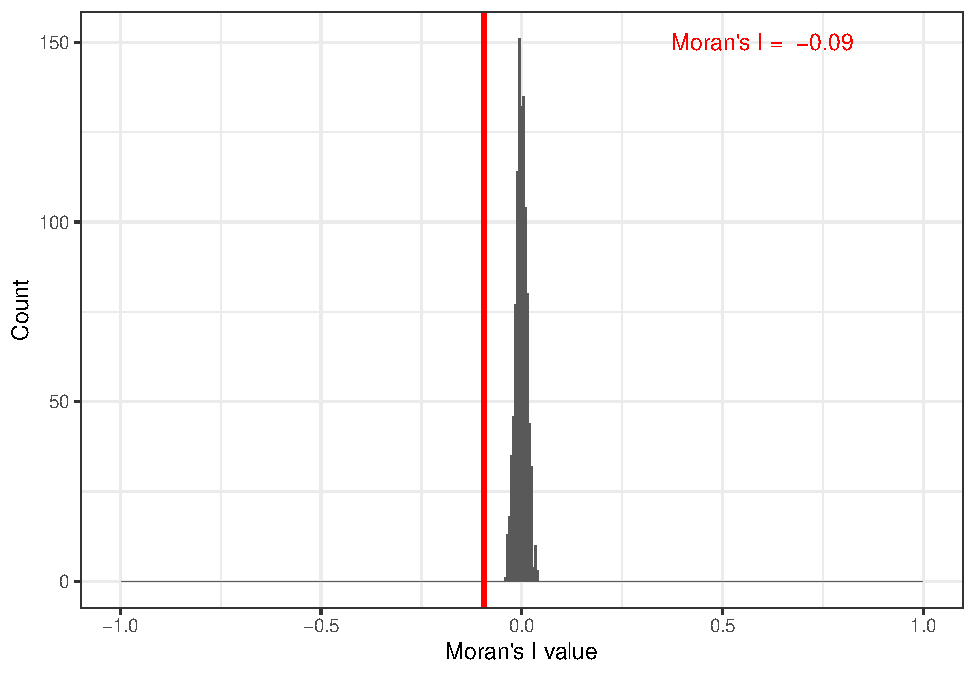
\includegraphics{HW2-SpatialRegression_files/figure-latex/unnamed-chunk-7-1.pdf}
The Moran's I value of the spatial error model is -0.09, which is an
improvement over the Moran's I value of the OLS model at 0.31. The
spatial error model better accounts for spatial autocorrelation in the
data and shows less spatial autocorrelation in the residuals compared to
the OLS model. Our comparison criteria show that the spatial error model
appears to better account for spatial autocorrelation in our data
compared to the OLS model. The spatial error model has a lower AIC
value, higher log likelihood value, statistically significant likelihood
ratio test, and lower Moran's I value. However, the Breusch-Pagan test
shows that there is still heteroscedasticity present in the model's
residuals.

\hypertarget{comparison-between-spatial-regression-models}{%
\subsubsection{Comparison Between Spatial Regression
Models}\label{comparison-between-spatial-regression-models}}

We can compare the results of our spatial regression models based on the
values of the AIC/SC results. The spatial lag regression's AIC value of
525 is lower than the spatial error regression's AIC value of 755,
indicating that the the spatial lag model is a better spatial regression
model for our data.

\hypertarget{geographically-weighted-regression}{%
\subsection{Geographically Weighted
Regression}\label{geographically-weighted-regression}}

\begin{Shaded}
\begin{Highlighting}[]
\CommentTok{\#Setting an adaptive bandwidth}
\NormalTok{datas }\OtherTok{\textless{}{-}} \FunctionTok{as}\NormalTok{(data, }\StringTok{\textquotesingle{}Spatial\textquotesingle{}}\NormalTok{)  }\CommentTok{\#These analyses are easier to do when the data are of the SpatialPolygonsDataFrame class}
\FunctionTok{class}\NormalTok{ (datas)}
\end{Highlighting}
\end{Shaded}

\begin{verbatim}
## [1] "SpatialPolygonsDataFrame"
## attr(,"package")
## [1] "sp"
\end{verbatim}

\begin{Shaded}
\begin{Highlighting}[]
\NormalTok{bw}\OtherTok{\textless{}{-}}\FunctionTok{gwr.sel}\NormalTok{(}\AttributeTok{formula=}\NormalTok{LNMEDHVAL }\SpecialCharTok{\textasciitilde{}}\NormalTok{ LNNBELPOV }\SpecialCharTok{+}\NormalTok{ PCTBACHMOR }\SpecialCharTok{+}\NormalTok{ PCTSINGLES }\SpecialCharTok{+}\NormalTok{ PCTVACANT,}
            \AttributeTok{data=}\NormalTok{datas,}
            \AttributeTok{method =} \StringTok{"aic"}\NormalTok{,}
            \AttributeTok{adapt =} \ConstantTok{TRUE}\NormalTok{)}
\end{Highlighting}
\end{Shaded}

\begin{verbatim}
## Bandwidth: 0.381966 AIC: 1278.637 
## Bandwidth: 0.618034 AIC: 1333.984 
## Bandwidth: 0.236068 AIC: 1209.441 
## Bandwidth: 0.145898 AIC: 1115.788 
## Bandwidth: 0.09016994 AIC: 1007.261 
## Bandwidth: 0.05572809 AIC: 910.3448 
## Bandwidth: 0.03444185 AIC: 821.2049 
## Bandwidth: 0.02128624 AIC: 737.5153 
## Bandwidth: 0.01315562 AIC: 681.5228 
## Bandwidth: 0.008130619 AIC: 660.7924 
## Bandwidth: 0.005024999 AIC: 714.1722 
## Bandwidth: 0.009856235 AIC: 666.9998 
## Bandwidth: 0.006944377 AIC: 667.5033 
## Bandwidth: 0.008427513 AIC: 661.6706 
## Bandwidth: 0.007677515 AIC: 663.5923 
## Bandwidth: 0.008171309 AIC: 660.8446 
## Bandwidth: 0.008052658 AIC: 661.0577 
## Bandwidth: 0.008130619 AIC: 660.7924
\end{verbatim}

\hypertarget{results-1}{%
\subsubsection{Results}\label{results-1}}

The output shows the results of the GWR analysis in which the median
home value by block group is regressed against our four predictors. The
quasi global \(R^2\) value is 0.847 for the GWR analysis, the \(R^2\)
value for the OLS regression analysis is 0.6623. The GWR regression has
a higher \(R^2\) and appears to be better at explaining the variance in
the natural log of the median home sale value by block group.

\begin{Shaded}
\begin{Highlighting}[]
\NormalTok{gwrmodel}\OtherTok{\textless{}{-}}\FunctionTok{gwr}\NormalTok{(}\AttributeTok{formula=}\NormalTok{LNMEDHVAL }\SpecialCharTok{\textasciitilde{}}\NormalTok{ LNNBELPOV }\SpecialCharTok{+}\NormalTok{ PCTBACHMOR }\SpecialCharTok{+}\NormalTok{ PCTSINGLES }\SpecialCharTok{+}\NormalTok{ PCTVACANT,}
            \AttributeTok{data=}\NormalTok{datas,}
            \AttributeTok{adapt =}\NormalTok{ bw, }\CommentTok{\#adaptive bandwidth determined by proportion of observations accounted for}
            \AttributeTok{gweight=}\NormalTok{gwr.Gauss,}
            \AttributeTok{se.fit=}\ConstantTok{TRUE}\NormalTok{, }\CommentTok{\#to return local standard errors}
            \AttributeTok{hatmatrix =} \ConstantTok{TRUE}\NormalTok{)}
\NormalTok{gwrmodel}
\end{Highlighting}
\end{Shaded}

\begin{verbatim}
## Call:
## gwr(formula = LNMEDHVAL ~ LNNBELPOV + PCTBACHMOR + PCTSINGLES + 
##     PCTVACANT, data = datas, gweight = gwr.Gauss, adapt = bw, 
##     hatmatrix = TRUE, se.fit = TRUE)
## Kernel function: gwr.Gauss 
## Adaptive quantile: 0.008130619 (about 13 of 1720 data points)
## Summary of GWR coefficient estimates at data points:
##                    Min.    1st Qu.     Median    3rd Qu.       Max.  Global
## X.Intercept.  9.6727618 10.7143173 10.9542384 11.1742009 12.0831381 11.1138
## LNNBELPOV    -0.2365244 -0.0733572 -0.0401186 -0.0126657  0.0948768 -0.0789
## PCTBACHMOR    0.0010974  0.0101380  0.0149279  0.0202187  0.0347258  0.0209
## PCTSINGLES   -0.0249706 -0.0075550 -0.0016626  0.0042280  0.0143340  0.0030
## PCTVACANT    -0.0317407 -0.0142383 -0.0089599 -0.0035770  0.0167916 -0.0192
## Number of data points: 1720 
## Effective number of parameters (residual: 2traceS - traceS'S): 360.5225 
## Effective degrees of freedom (residual: 2traceS - traceS'S): 1359.477 
## Sigma (residual: 2traceS - traceS'S): 0.2762201 
## Effective number of parameters (model: traceS): 257.9061 
## Effective degrees of freedom (model: traceS): 1462.094 
## Sigma (model: traceS): 0.2663506 
## Sigma (ML): 0.245571 
## AICc (GWR p. 61, eq 2.33; p. 96, eq. 4.21): 660.7924 
## AIC (GWR p. 96, eq. 4.22): 308.7123 
## Residual sum of squares: 103.7248 
## Quasi-global R2: 0.8479244
\end{verbatim}

\hypertarget{akaike-information-criteria-aic}{%
\subsubsection{Akaike Information Criteria
(AIC)}\label{akaike-information-criteria-aic}}

The table below shows the AIC values for each of our four models. Models
with a lower AIC value have a better fit. Based on the AIC values, we
can conclude that the GWR model seems to be doing the best job
predicting the natural log of the median home value.

\begin{Shaded}
\begin{Highlighting}[]
\NormalTok{aic\_vector }\OtherTok{=} \FunctionTok{c}\NormalTok{(gwrmodel}\SpecialCharTok{$}\NormalTok{results}\SpecialCharTok{$}\NormalTok{AICh, lagreg}\SpecialCharTok{$}\NormalTok{AIC\_lm.model,}\FloatTok{525.48}\NormalTok{,}\FloatTok{754.985}\NormalTok{)}
\NormalTok{analysis\_vector }\OtherTok{=} \FunctionTok{c}\NormalTok{(}\StringTok{"GWR"}\NormalTok{,}\StringTok{"OLS"}\NormalTok{,}\StringTok{"Spatial Lag"}\NormalTok{,}\StringTok{"Spatial Error"}\NormalTok{)}

\FunctionTok{data.frame}\NormalTok{(analysis\_vector,aic\_vector) }\SpecialCharTok{\%\textgreater{}\%}
  \FunctionTok{kbl}\NormalTok{(}\AttributeTok{col.names=}\FunctionTok{c}\NormalTok{(}\StringTok{"Model"}\NormalTok{,}\StringTok{"AIC"}\NormalTok{)) }\SpecialCharTok{\%\textgreater{}\%}
  \FunctionTok{kable\_classic\_2}\NormalTok{()}
\end{Highlighting}
\end{Shaded}

\begin{table}
\centering
\begin{tabular}[t]{l|r}
\hline
Model & AIC\\
\hline
GWR & 308.7123\\
\hline
OLS & 1434.9867\\
\hline
Spatial Lag & 525.4800\\
\hline
Spatial Error & 754.9850\\
\hline
\end{tabular}
\end{table}

\hypertarget{geographically-weighted-regression-morans-i-results}{%
\subsubsection{Geographically Weighted Regression Moran's I
Results}\label{geographically-weighted-regression-morans-i-results}}

The plot below shows the global Moran's I value for the residuals of the
Geographic Weighted Regression. The global Moran's I value of the GWR
residuals is 0.03. By comparing the Moran's I value to the histogram of
random permutations we can conclude that there is clustering in the GWR
residuals. However, there is a slight possibility that this clustering
is the result of random chance as a small number of the random Moran's I
permutations have Moran's I values which are higher than 0.03. The
p-value for the Moran's I statistic of the GWR residuals is 0.014,
indicating that we are only 97.2\% confident the clustering is not the
result of random chance and there is a very small possibility the
clustering of the GWR residuals could be random. When compared to other
models, the GWR residuals are less clustered than the OLS residuals. The
Spatial Lag and Spatial Error residuals have negative Moran's I value
indicating spatial dispersion (i.e: negative spatial autocorrelation).
Because the absolute value of the Moran's I statistic for the GWR
regression is lower than the other three models, we can conclude that
the residuals of the GWR regression have the least amount of spatial
autocorrelation.

\begin{Shaded}
\begin{Highlighting}[]
\NormalTok{gwrMoranMc}\OtherTok{\textless{}{-}}\FunctionTok{moran.mc}\NormalTok{(gwrmodel}\SpecialCharTok{$}\NormalTok{SDF}\SpecialCharTok{@}\NormalTok{data}\SpecialCharTok{$}\NormalTok{gwr.e, queenlist, }\DecValTok{999}\NormalTok{, }\AttributeTok{alternative=}\StringTok{"two.sided"}\NormalTok{)}

\CommentTok{\#Draws distribution of Moran\textquotesingle{}s I\textquotesingle{}s calculated from randomly permuted values}
\CommentTok{\# Here, we draw a red vertical line at the observed value of our Moran\textquotesingle{}s I}

\FunctionTok{ggplot}\NormalTok{()}\SpecialCharTok{+}
  \FunctionTok{geom\_histogram}\NormalTok{(}\FunctionTok{aes}\NormalTok{(gwrMoranMc}\SpecialCharTok{$}\NormalTok{res),}\AttributeTok{binwidth =} \FloatTok{0.005}\NormalTok{)}\SpecialCharTok{+}
  \FunctionTok{xlim}\NormalTok{(}\SpecialCharTok{{-}}\DecValTok{1}\NormalTok{,}\DecValTok{1}\NormalTok{)}\SpecialCharTok{+}
  \FunctionTok{geom\_vline}\NormalTok{(}\AttributeTok{xintercept=}\NormalTok{gwrMoranMc}\SpecialCharTok{$}\NormalTok{statistic,}\AttributeTok{color=}\StringTok{\textquotesingle{}red\textquotesingle{}}\NormalTok{,}\AttributeTok{linewidth=}\DecValTok{1}\NormalTok{)}\SpecialCharTok{+}
  \FunctionTok{annotate}\NormalTok{(}\StringTok{"text"}\NormalTok{,}\AttributeTok{x=}\FloatTok{0.6}\NormalTok{, }\AttributeTok{y=}\DecValTok{150}\NormalTok{,}\AttributeTok{color=}\StringTok{\textquotesingle{}red\textquotesingle{}}\NormalTok{,}\AttributeTok{label=}\FunctionTok{paste}\NormalTok{(}\StringTok{"Moran\textquotesingle{}s I = "}\NormalTok{,}\FunctionTok{as.character}\NormalTok{(}\FunctionTok{round}\NormalTok{(gwrMoranMc}\SpecialCharTok{$}\NormalTok{statistic,}\DecValTok{2}\NormalTok{))))}\SpecialCharTok{+}
  \FunctionTok{labs}\NormalTok{(}\AttributeTok{x=}\StringTok{"Moran\textquotesingle{}s I value"}\NormalTok{,}\AttributeTok{y=}\StringTok{\textquotesingle{}Count\textquotesingle{}}\NormalTok{)}\SpecialCharTok{+}
  \FunctionTok{theme\_bw}\NormalTok{()}
\end{Highlighting}
\end{Shaded}

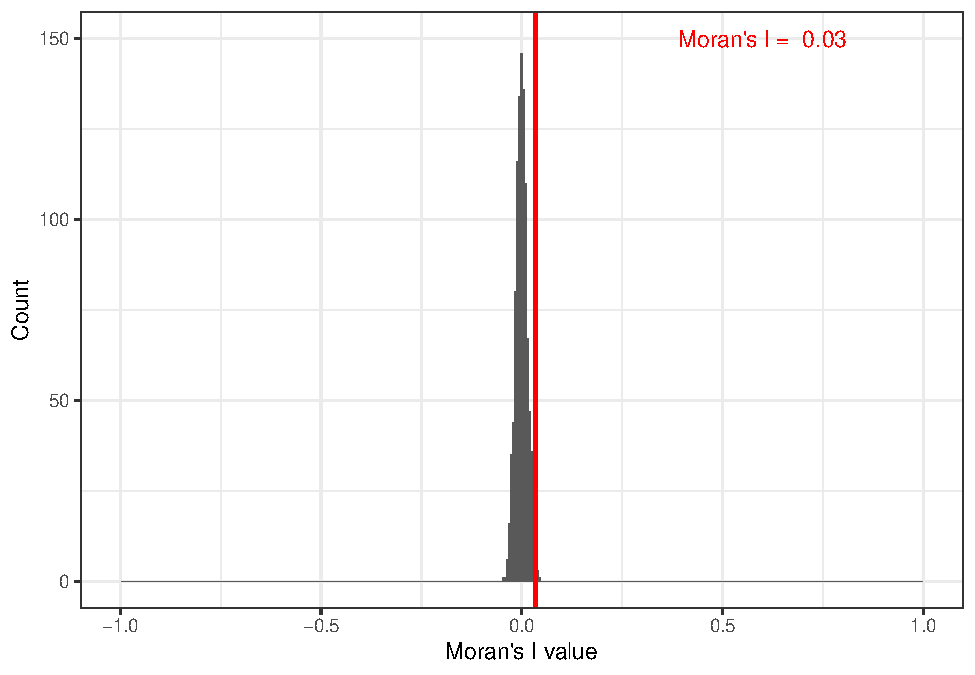
\includegraphics{HW2-SpatialRegression_files/figure-latex/unnamed-chunk-10-1.pdf}

\hypertarget{gwr-local-regression-results}{%
\subsubsection{GWR Local Regression
Results}\label{gwr-local-regression-results}}

The maps below show the beta coefficient divided by the standard error
for each of our four dependent variables. This figure is referred to as
a standardized coefficient. If the standardized coefficient is greater
than two we can conclude that there is possibly a significant local
positive relationship between the predictor and the natural log of the
median home sales value. If the coefficient is less than negative two we
can conclude that there is possibly a significant negative relationship
between the predictor and the natural log of the median home sale value.
From the maps below, we can conclude that there is a possibly
significant positive relationship between the percent of households with
a bachelors degree and the natural log of median home sale value in most
of the city. There is also possibly a statistically significant negative
relationship between the percent of Houses which are vacant and the
natural log of the median home sale value in many parts of Philadelphia
including areas of Northwest Philadelphia, South Philadelphia, and parts
of West Philadelphia. There is a possibly statistically significant
positive relationship between the Percent of Single Family Houses and
the natural log of the median home values in large sections of Northeast
and Northwest Philadelphia. This possibly significant positive
relationship is not present in other parts of Philadelphia where the
number of single family homes tends to be smaller.

\begin{Shaded}
\begin{Highlighting}[]
\NormalTok{gwrresults}\OtherTok{\textless{}{-}}\FunctionTok{as.data.frame}\NormalTok{(gwrmodel}\SpecialCharTok{$}\NormalTok{SDF)}

\NormalTok{data}\SpecialCharTok{$}\NormalTok{coefLNNBELPOVst}\OtherTok{\textless{}{-}}\NormalTok{gwrresults}\SpecialCharTok{$}\NormalTok{LNNBELPOV}\SpecialCharTok{/}\NormalTok{gwrresults}\SpecialCharTok{$}\NormalTok{LNNBELPOV\_se}
\NormalTok{data}\SpecialCharTok{$}\NormalTok{coefPCTBACHMORst}\OtherTok{\textless{}{-}}\NormalTok{gwrresults}\SpecialCharTok{$}\NormalTok{PCTBACHMOR}\SpecialCharTok{/}\NormalTok{gwrresults}\SpecialCharTok{$}\NormalTok{PCTBACHMOR\_se}
\NormalTok{data}\SpecialCharTok{$}\NormalTok{coefPCTSINGLESst}\OtherTok{\textless{}{-}}\NormalTok{gwrresults}\SpecialCharTok{$}\NormalTok{PCTSINGLES}\SpecialCharTok{/}\NormalTok{gwrresults}\SpecialCharTok{$}\NormalTok{PCTSINGLES\_se}
\NormalTok{data}\SpecialCharTok{$}\NormalTok{coefPCTVACANTst}\OtherTok{\textless{}{-}}\NormalTok{gwrresults}\SpecialCharTok{$}\NormalTok{PCTVACANT}\SpecialCharTok{/}\NormalTok{gwrresults}\SpecialCharTok{$}\NormalTok{PCTVACANT\_se}

\NormalTok{coefLNNBELPOV}\OtherTok{\textless{}{-}}\FunctionTok{tm\_shape}\NormalTok{(data)}\SpecialCharTok{+}
  \FunctionTok{tm\_fill}\NormalTok{(}\AttributeTok{col=}\StringTok{\textquotesingle{}coefLNNBELPOVst\textquotesingle{}}\NormalTok{, }\AttributeTok{breaks=}\FunctionTok{c}\NormalTok{(}\SpecialCharTok{{-}}\ConstantTok{Inf}\NormalTok{, }\SpecialCharTok{{-}}\DecValTok{2}\NormalTok{, }\DecValTok{0}\NormalTok{, }\DecValTok{2}\NormalTok{, }\ConstantTok{Inf}\NormalTok{), }\AttributeTok{title=}\StringTok{\textquotesingle{}Standardized coef. of LNNBELPOV\textquotesingle{}}\NormalTok{, }
          \AttributeTok{palette =}\StringTok{\textquotesingle{}{-}RdBu\textquotesingle{}}\NormalTok{)}\SpecialCharTok{+}
  \FunctionTok{tm\_layout}\NormalTok{(}\AttributeTok{frame=}\ConstantTok{FALSE}\NormalTok{, }\AttributeTok{title =} \StringTok{\textquotesingle{}Number Below Poverty (Log)\textquotesingle{}}\NormalTok{)}

\NormalTok{coefPCTBACHMOR}\OtherTok{\textless{}{-}}\FunctionTok{tm\_shape}\NormalTok{(data)}\SpecialCharTok{+}
  \FunctionTok{tm\_fill}\NormalTok{(}\AttributeTok{col=}\StringTok{\textquotesingle{}coefPCTBACHMORst\textquotesingle{}}\NormalTok{, }\AttributeTok{breaks=}\FunctionTok{c}\NormalTok{(}\SpecialCharTok{{-}}\ConstantTok{Inf}\NormalTok{, }\SpecialCharTok{{-}}\DecValTok{2}\NormalTok{, }\DecValTok{0}\NormalTok{, }\DecValTok{2}\NormalTok{, }\ConstantTok{Inf}\NormalTok{), }\AttributeTok{title=}\StringTok{\textquotesingle{}Standardized coef. of PCTBACHMOR\textquotesingle{}}\NormalTok{, }
          \AttributeTok{palette=}\StringTok{\textquotesingle{}{-}RdBu\textquotesingle{}}\NormalTok{)}\SpecialCharTok{+}
  \FunctionTok{tm\_layout}\NormalTok{(}\AttributeTok{frame=}\ConstantTok{FALSE}\NormalTok{, }\AttributeTok{title =} \StringTok{\textquotesingle{}Pct. of Bachelors or Higher\textquotesingle{}}\NormalTok{)}

\NormalTok{coefPCTSINGLES}\OtherTok{\textless{}{-}}\FunctionTok{tm\_shape}\NormalTok{(data)}\SpecialCharTok{+}
  \FunctionTok{tm\_fill}\NormalTok{(}\AttributeTok{col=}\StringTok{\textquotesingle{}coefPCTSINGLESst\textquotesingle{}}\NormalTok{, }\AttributeTok{breaks=}\FunctionTok{c}\NormalTok{(}\SpecialCharTok{{-}}\ConstantTok{Inf}\NormalTok{, }\SpecialCharTok{{-}}\DecValTok{2}\NormalTok{, }\DecValTok{0}\NormalTok{, }\DecValTok{2}\NormalTok{, }\ConstantTok{Inf}\NormalTok{), }\AttributeTok{title=}\StringTok{\textquotesingle{}Standardized coef. of PCTSINGLES\textquotesingle{}}\NormalTok{, }
          \AttributeTok{palette=}\StringTok{\textquotesingle{}{-}RdBu\textquotesingle{}}\NormalTok{)}\SpecialCharTok{+}
  \FunctionTok{tm\_layout}\NormalTok{(}\AttributeTok{frame=}\ConstantTok{FALSE}\NormalTok{, }\AttributeTok{title =} \StringTok{\textquotesingle{}Pct. of Single Family Houses\textquotesingle{}}\NormalTok{)}

\NormalTok{coefPCTVACANT}\OtherTok{\textless{}{-}}\FunctionTok{tm\_shape}\NormalTok{(data)}\SpecialCharTok{+}
  \FunctionTok{tm\_fill}\NormalTok{(}\AttributeTok{col=}\StringTok{\textquotesingle{}coefPCTVACANTst\textquotesingle{}}\NormalTok{, }\AttributeTok{breaks=}\FunctionTok{c}\NormalTok{(}\SpecialCharTok{{-}}\ConstantTok{Inf}\NormalTok{, }\SpecialCharTok{{-}}\DecValTok{2}\NormalTok{, }\DecValTok{0}\NormalTok{, }\DecValTok{2}\NormalTok{, }\ConstantTok{Inf}\NormalTok{), }\AttributeTok{title=}\StringTok{\textquotesingle{}Standardized coef. of PCTVACANT\textquotesingle{}}\NormalTok{, }
          \AttributeTok{palette=}\StringTok{\textquotesingle{}{-}RdBu\textquotesingle{}}\NormalTok{)}\SpecialCharTok{+}
  \FunctionTok{tm\_layout}\NormalTok{(}\AttributeTok{frame=}\ConstantTok{FALSE}\NormalTok{, }\AttributeTok{title =} \StringTok{\textquotesingle{}Pct. of Housing Vacant\textquotesingle{}}\NormalTok{)}

\FunctionTok{tmap\_arrange}\NormalTok{(coefLNNBELPOV,coefPCTBACHMOR, coefPCTSINGLES, coefPCTVACANT, }\AttributeTok{ncol=}\DecValTok{2}\NormalTok{)}
\end{Highlighting}
\end{Shaded}

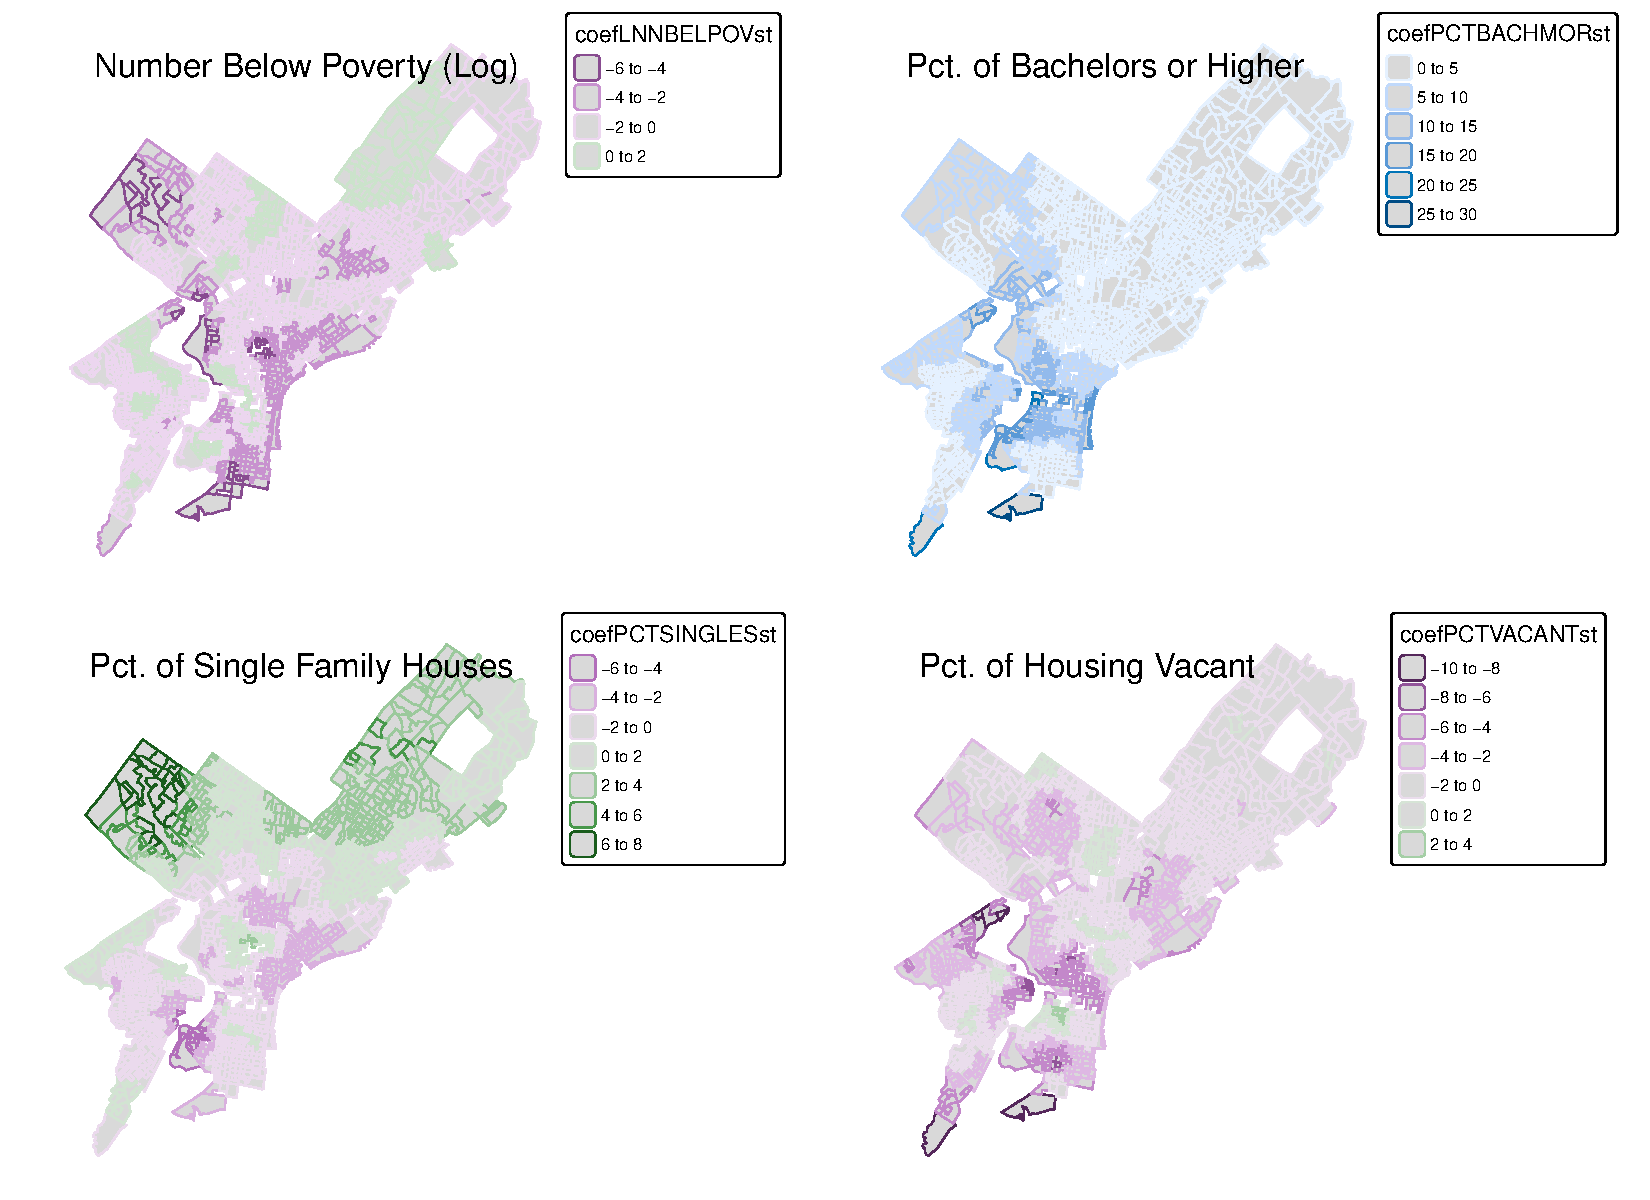
\includegraphics{HW2-SpatialRegression_files/figure-latex/unnamed-chunk-11-1.pdf}

\hypertarget{local-r2-map}{%
\subsubsection{Local R2 Map}\label{local-r2-map}}

The map below shows the local \(R^2\) values for the GWR regression. In
areas where the \(R^2\) is higher our local regression model explains
more of the variation in median home sales values. The Local \(R^2\) for
most block groups in South Philadelphia, Northwest Philadelphia, and
Northeast Philadelphia is greater than 0.5 indicating our model does a
good job explaining the variance of the dependent variable. However,
there are localized areas of North Philadelphia and West Philadelphia
where the \(R^2\) is less than 0.2 indicating that the model does not do
a good job explaining the variance in the median home sale value.

\begin{Shaded}
\begin{Highlighting}[]
\NormalTok{data}\SpecialCharTok{$}\NormalTok{localR2 }\OtherTok{\textless{}{-}}\NormalTok{ gwrmodel}\SpecialCharTok{$}\NormalTok{SDF}\SpecialCharTok{$}\NormalTok{localR2}

\FunctionTok{tm\_shape}\NormalTok{(data)}\SpecialCharTok{+}
  \FunctionTok{tm\_fill}\NormalTok{(}\AttributeTok{col=}\StringTok{\textquotesingle{}localR2\textquotesingle{}}\NormalTok{,  }\AttributeTok{breaks=}\FunctionTok{c}\NormalTok{(}\DecValTok{0}\NormalTok{, }\FloatTok{0.1}\NormalTok{, }\FloatTok{0.2}\NormalTok{, }\FloatTok{0.3}\NormalTok{, }\FloatTok{0.4}\NormalTok{, }\FloatTok{0.5}\NormalTok{, }\FloatTok{0.6}\NormalTok{, }\FloatTok{0.7}\NormalTok{), }\AttributeTok{n=}\DecValTok{5}\NormalTok{, }\AttributeTok{palette =} \StringTok{\textquotesingle{}Blues\textquotesingle{}}\NormalTok{)}\SpecialCharTok{+}
  \FunctionTok{tm\_layout}\NormalTok{(}\AttributeTok{frame=}\ConstantTok{FALSE}\NormalTok{)}
\end{Highlighting}
\end{Shaded}

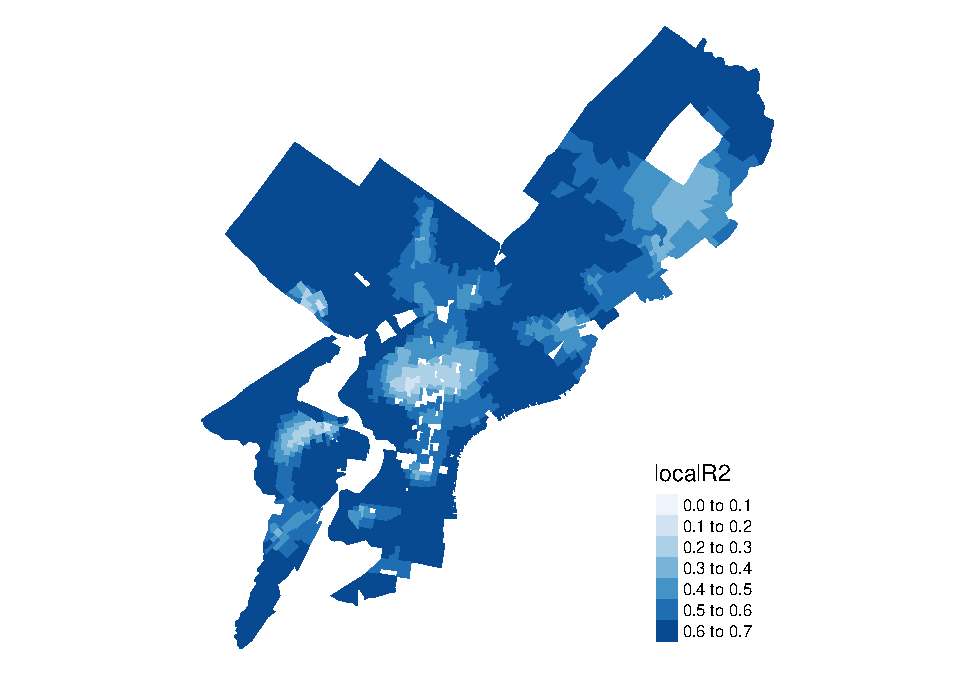
\includegraphics{HW2-SpatialRegression_files/figure-latex/local R2 map-1.pdf}

\hypertarget{discussion}{%
\section{Discussion}\label{discussion}}

Through this analysis, we built upon our previous multiple regression
analysis of median home values in Philadelphia through spatial
regression techniques to account for spatial autocorrelation in the
data. This report explores multiple spatial regression techniques,
including spatial lag regression, spatial error regression, and
geographically weighted regression, to examine which technique best fits
our Philadelphia data set. We can conclude that spatial regression
techniques do provide a better model fit for our data compared to OLS
regression based on the comparisons of different model metrics. The GWR
model had the lowest AIC value and a Moran's I value that was closest to
0, which means the model was the most effective at accounting for
spatial autocorrelation out of the four regression techniques presented
in this analysis.

The spatial lag and spatial error methods have statistically significant
values for their Breusch Pagan tests, which indicate that the residuals
still show the heteroscedasticity that the OLS model does. Having
homoscedastic residuals remains an important assumption for running
these models, so these methods do not account for this assumption.

While GWR does have a lowest AIC, the model performance is mixed and the
predictors we use do a good job accounting for the variation in mean
household value in some neighborhoods but not others. Notably, the GWR
model appears to do a very poor job explaining the variation in median
home sale prices in areas with a large minority population like North
Philadelphia and West Philadelphia. Additionally, local GWR regressions
predictors are likely to display some degree of local multicollinearity.
For example, the proportion of residents in a block group with at least
a bachelor's degree and the proportion of homes which are single family
homes are likely to be collinear in parts of Northwest Philadelphia even
though they are not collinear at a city side scale.

Spatially weighted residuals (i.e., spatially lagged) are the residuals
from a regression model that have been adjusted for spatial
autocorrelation. These residuals are weighted based on a spatial weights
matrix (Queen's neighbor). Spatially lagged residuals show how
observations may be related to neighboring observations. In contrast a
spatial lag model directly incorporates spatial dependance into
regression through a spatially lagged dependent variable. Meaning, that
the dependent variable for one observation is explained not only by its
own predictors but also by the values of the dependent variable for its
neighbors. The residuals from a spatial lag model are the differences
between the observed values of the dependent variable and the values
predicted by the model, which includes this spatially lagged dependent
variable. Spatial lag model residuals are expected to show less spatial
autocorrelation than ordinary least squares residuals because the model
itself accounts for spatial dependence.

ArcGIS Pro, an industry standard for GIS and spatial analysis, is
problematic to use for GWR models because it uses unclear methodologies
to run the regression and returns either unhelpful or nonsensical
results. Instead of an AIC value, ArcGIS Pro only returns an AIC
corrected (AICc) value, which cannot be used to compare with AIC outputs
for other regression methods. ArcGIS Pro optimizes bandwidth for the
model using a confusing methodology called Golden search, and can return
outputs that include negative R\^{}2 values, which should be instead
bounded between zero and one. Other tools, such as R, are a more
consistent and appropriate choice to use when developing a GWR model.

\end{document}
